\definecolor{c10p1blue}{HTML}{2A78D6}
\definecolor{c10p1orange}{HTML}{EB6834}
\definecolor{c10p1aqua}{HTML}{1BAF7A}
\definecolor{c10p1gray}{HTML}{52514E}

\section{The welfare value of a new good: virtual prices and exact measures}\label{sec:10-virtual}

A new good raises welfare because consumers can buy something they could not buy before. This section turns
that statement into a number. Following \citet{Hicks1940}, we treat the period before the introduction as a
period in which the good is rationed at zero. The value of the good is then the compensating variation of
raising its price from the observed level to its \emph{virtual price}. At that price the consumer would
choose not to buy the good. We derive this result, relate it to the exact cost-of-living index of
\citet{Konus1939}, and show why price indexes that link new goods in after their introduction miss it. We
then derive index-number bounds, state what separability buys, and derive the variety correction of
\citet{Feenstra1994}. The duality tools come from \cref{sec:05-duality}, and \cref{sec:05-welfare-virtual}
treats virtual prices for the almost ideal demand system.

\subsection{Setting and notation}\label{sec:10-setting}

A consumer chooses quantities $q = (q_1,\dots,q_n)^\top \ge 0$ of $n$ goods at prices
$p = (p_1,\dots,p_n)^\top$, all positive, with income $y$. We write $q_j(p,y)$ for Marshallian demand,
$v(p,y)$ for indirect utility, $e(p,u)$ for the expenditure function and $h_j(p,u)$ for Hicksian demand.
Good $n$ is the new good. It is unavailable in period 0 and sold at price $p_n$ in period 1. We write
$p_{-n}$ for the prices of the other goods and $(p_{-n},p_n)$ for the full price vector. Following
\citet{Hausman1997} and \citet{Petrin2002} we write income as $y$. \Cref{ch:aids} writes $I$ for the same
object.

\begin{assumption}[Preferences]\label{ass:10-prefs}
The utility function $U$ is continuous, strictly increasing and strictly quasi-concave on $\R^n_+$.
\end{assumption}

Under Assumption~\ref{ass:10-prefs} demands are single valued and continuous, and the duality identities of
\cref{lem:05-duality} hold:
\begin{equation}\label{eq:10-duality}
  e\bigl(p,v(p,y)\bigr) = y, \qquad h_j(p,u) = q_j\bigl(p,e(p,u)\bigr), \qquad
  \frac{\partial e(p,u)}{\partial p_j} = h_j(p,u).
\end{equation}
The last identity is Shephard's lemma (\cref{prop:05-shephard}). The expenditure function is nondecreasing
and concave in $p$, so each Hicksian demand is nonincreasing in its own price (\cref{prop:05-e-properties}).

\subsection{A new good as a rationed good}\label{sec:10-rationing}

\citet{Hicks1940} treated rationing and new goods with the same tool. As \citet[p.~211]{Hausman1997} puts it,
new products are a special case of rationing in which demand for the good is zero. Before the introduction, the consumer solves the usual problems with the extra
constraint $q_n = 0$. We call the resulting value functions the \emph{rationed} indirect utility and
expenditure functions:
\begin{align}
  v^R(p_{-n},y) &= \max\Bigl\{U(q) : \sum_{j\neq n}p_jq_j \le y,\ q_n = 0\Bigr\}, \label{eq:10-vR}\\
  e^R(p_{-n},u) &= \min\Bigl\{\sum_{j\neq n}p_jq_j : U(q) \ge u,\ q_n = 0\Bigr\}. \label{eq:10-eR}
\end{align}
Neither function depends on $p_n$, because a bundle with $q_n = 0$ costs the same at every price of good $n$.
\Cref{sec:05-welfare-virtual} writes $e_{-i}$ for $e^R$.

\begin{definition}[Virtual prices]\label{def:10-virtual}
The \emph{Hicksian virtual price} $p_n^V(p_{-n},u)$ of good $n$ is the virtual price of \cref{def:05-virtual},
the lowest price at which Hicksian demand $h_n$ is zero. The \emph{Marshallian virtual price} (or choke price) is
the same object for Marshallian demand, $p_n^M(p_{-n},y) = \inf\{p_n > 0 : q_n(p_{-n},p_n,y) = 0\}$. Either
price is $+\infty$ if the corresponding demand is positive at every price.
\end{definition}

In both cases demand stays at zero at every price above the virtual price. For Hicksian demand this follows
because $h_n$ is nonincreasing in $p_n$. For Marshallian demand, suppose the optimal bundle at $p_n$ has
$q_n = 0$. Raising $p_n$ leaves its cost unchanged and shrinks the budget set, so the same bundle stays
optimal. \citet[p.~212, n.~5]{Hausman1997} uses the Hicksian version, because the exact welfare measure keeps
utility constant. The two versions coincide when demand for good $n$ has no income effect. For a normal good
the Hicksian virtual price at the period-1 utility is at least the Marshallian one (\cref{lem:05-choke-order}).

The next lemma is the formal content of the virtual-price idea. \citet{Rothbarth1941} introduced it, and
\citet{NearyRoberts1980} give a modern treatment of rationing along these lines. \citet[Section~4.3,
pp.~109--113]{DeatonMuellbauer1980b} give the textbook treatment through the restricted cost function, which
\cref{lem:10-restricted} below develops.

\begin{lemma}[Rationing as a price, \citealp{Rothbarth1941,NearyRoberts1980}]\label{lem:10-rothbarth}
Let Assumption~\ref{ass:10-prefs} hold and fix $p_{-n}$, $y$ and $u$.
\begin{enumerate}[label=(\alph*)]
  \item For every $p_n > 0$, $v(p_{-n},p_n,y) \ge v^R(p_{-n},y)$ and $e(p_{-n},p_n,u) \le e^R(p_{-n},u)$.
  \item If $p_n^M(p_{-n},y)$ is finite, then $v^R(p_{-n},y) = v\bigl(p_{-n},p_n^M(p_{-n},y),y\bigr)$.
  \item If $p_n^V(p_{-n},u)$ is finite, then $e^R(p_{-n},u) = e\bigl(p_{-n},p_n^V(p_{-n},u),u\bigr)$.
\end{enumerate}
\end{lemma}

\begin{proof}
(a) Any bundle that is feasible in the rationed problem has $q_n = 0$. Its cost is therefore the same at
every $p_n$, and it is feasible in the unrationed problem at every $p_n$. Maximizing over a larger set gives
a weakly larger maximum, and minimizing over a larger set gives a weakly smaller minimum.

(b) Write $p_n^M$ for $p_n^M(p_{-n},y)$ and let $q^* = q(p_{-n},p_n^M,y)$. Marshallian demand is continuous
in prices, so $q_n^* = 0$ at the infimum in \cref{def:10-virtual}. Hence
$\sum_{j\neq n}p_jq_j^* = p^\top q^* \le y$, and $q^*$ is feasible in the rationed problem. This gives
$v^R(p_{-n},y) \ge U(q^*) = v(p_{-n},p_n^M,y)$. Part (a) at $p_n = p_n^M$ gives the reverse inequality.

(c) The argument is the same with $h(p_{-n},p_n^V,u)$ in place of $q^*$. Its $n$th component is zero, so it
is feasible in the rationed cost minimization, and $e^R(p_{-n},u) \le e(p_{-n},p_n^V,u)$. Part (a) gives the
reverse inequality.
\end{proof}

\begin{remark}[The virtual price as a shadow price]\label{rem:10-shadow}
Suppose $U$ is differentiable, the good would be bought at the actual price, and the rationed optimum $q^R$
has $q_j^R > 0$ for every $j \neq n$. Write the ration as $q_n \le 0$, with multiplier $\mu \ge 0$, and the
budget with multiplier $\lambda > 0$. The Kuhn-Tucker conditions are
\begin{align*}
  \frac{\partial U(q^R)}{\partial q_j} &= \lambda p_j, \qquad j \neq n, \\
  \frac{\partial U(q^R)}{\partial q_n} &= \lambda p_n + \mu = \lambda\Bigl(p_n + \frac{\mu}{\lambda}\Bigr).
\end{align*}
Define $\tilde p_n = p_n + \frac{\mu}{\lambda}$. The two lines are then the first-order conditions of the
unrationed problem at prices $(p_{-n},\tilde p_n)$. The budget is unchanged, because the ration contributes
$(\tilde p_n - p_n)\cdot 0 = 0$ to spending. Since the conditions are sufficient under strict
quasi-concavity, $q^R$ is the unrationed demand at $(p_{-n},\tilde p_n,y)$. The price $\tilde p_n$ equals the
marginal rate of substitution between good $n$ and money at $q^R$. It is the price at which the consumer is
just unwilling to buy the first unit, the Marshallian virtual price. The multiplier
$\mu = \lambda(p_n^M - p_n)$ is the utility value of relaxing the ration by one unit, and $\frac{\mu}{\lambda}$
is its money value. Rothbarth called such prices the ``virtual price system''
\citep[p.~211]{Hausman1997}.
\end{remark}

The remark finds the shadow price at the rationed optimum, holding income fixed. The welfare measures below hold
utility fixed, and for them it helps to treat the ration $q_n = z$ as a variable. The cost function with a fixed
quantity of one good is the consumer's analogue of a short-run cost function. The unrestricted cost function is its
long-run envelope \citep[p.~110]{DeatonMuellbauer1980b}.

\begin{lemma}[Restricted expenditure function, \citealp{DeatonMuellbauer1980b}]\label{lem:10-restricted}
Let Assumption~\ref{ass:10-prefs} hold and let $U$ be differentiable. For a ration $z \ge 0$ of good $n$, define
the \emph{restricted expenditure function}
\begin{equation}\label{eq:10-restricted}
  \tilde e(p,u,z) = \min\Bigl\{p^\top q : U(q) \ge u,\ q_n = z\Bigr\}
  = p_nz + \min_{q_{-n}}\Bigl\{\sum_{j\neq n}p_jq_j : U(q_{-n},z) \ge u\Bigr\}.
\end{equation}
\begin{enumerate}[label=(\alph*)]
  \item $e^R(p_{-n},u) = \tilde e(p,u,0)$, and $e(p,u) = \min_{z\ge 0}\tilde e(p,u,z)$, with the minimum at
  $z = h_n(p,u)$.
  \item Suppose the minimizing $q_{-n}$ in \eqref{eq:10-restricted} has $q_j > 0$ for every $j \neq n$, and let
  $\kappa > 0$ be the multiplier on the utility constraint. Define the \emph{shadow price} of the ration as
  $\tilde p_n(p_{-n},u,z) = \kappa\frac{\partial U}{\partial q_n}$. Then
  \begin{equation}\label{eq:10-restricted-deriv}
    \frac{\partial\tilde e(p,u,z)}{\partial z} = p_n - \tilde p_n(p_{-n},u,z),
  \end{equation}
  and $h_n\bigl(p_{-n},\tilde p_n(p_{-n},u,z),u\bigr) = z$.
\end{enumerate}
\end{lemma}

\begin{proof}
(a) With $z = 0$ the term $p_nz$ vanishes, and the problem in \eqref{eq:10-restricted} is the rationed problem
\eqref{eq:10-eR}. For the second claim, minimize $p^\top q$ subject to $U(q) \ge u$ in two steps. The first step
fixes $q_n = z$ and minimizes over $q_{-n}$, which gives $\tilde e(p,u,z)$. The second step minimizes over $z$. The
minimizing $z$ is the $n$th component of the cost-minimizing bundle, $h_n(p,u)$.

(b) Write $g(z)$ for the inner minimum in \eqref{eq:10-restricted}. Its Lagrangian is
\begin{equation*}
  \mathcal{L} = \sum_{j\neq n}p_jq_j - \kappa\bigl[U(q_{-n},z) - u\bigr].
\end{equation*}
At an interior optimum the first-order conditions are $p_j = \kappa\frac{\partial U}{\partial q_j}$ for $j \neq n$.
The envelope theorem gives
\begin{equation*}
  g'(z) = \frac{\partial\mathcal{L}}{\partial z} = -\kappa\frac{\partial U}{\partial q_n} = -\tilde p_n(p_{-n},u,z).
\end{equation*}
Adding the derivative of $p_nz$ gives \eqref{eq:10-restricted-deriv}. Now consider the unrestricted cost
minimization at prices $(p_{-n},\tilde p_n)$ and the bundle $(q_{-n},z)$. The conditions
$p_j = \kappa\frac{\partial U}{\partial q_j}$ hold for $j \neq n$ by construction. The condition for good $n$,
$\tilde p_n = \kappa\frac{\partial U}{\partial q_n}$, holds by the definition of $\tilde p_n$. Under
Assumption~\ref{ass:10-prefs} these conditions are sufficient. The bundle is therefore the Hicksian demand at
$(p_{-n},\tilde p_n,u)$, and its $n$th component is $z$.
\end{proof}

The shadow price is the money value of one more unit of the ration. It equals the fall in the cost of staying on
the indifference curve when that unit is supplied free \citep[p.~113]{DeatonMuellbauer1980b}. By part (b), the
function $z \mapsto \tilde p_n(p_{-n},u,z)$ is the inverse of the compensated demand curve for good $n$. At $z = 0$ it
is the price at which the consumer just chooses not to buy, the Hicksian counterpart of the shadow price in
\cref{rem:10-shadow}. The derivative \eqref{eq:10-restricted-deriv} vanishes at $z = h_n(p,u)$, which is the envelope
property of part (a). Deaton and Muellbauer state the three results as their equations (3.1), (3.2) and (3.7)
(pp.~110--112).

\subsection{The compensating variation of a new good}\label{sec:10-cv}

Hold income $y$ and the other prices $p_{-n}$ fixed across the two periods for now. Period-0 utility is
$u^0 = v^R(p_{-n},y)$ and period-1 utility is $u^1 = v(p_{-n},p_n,y)$. By \cref{lem:10-rothbarth}(a),
$u^1 \ge u^0$.

\begin{definition}[Value of a new good]\label{def:10-cv}
The \emph{compensating variation} of the new good is
\begin{equation}\label{eq:10-cv-def}
  CV = e^R(p_{-n},u^1) - y,
\end{equation}
the extra income a consumer without access to the good would need to reach the period-1 utility. The
\emph{equivalent variation} is $EV = y - e(p_{-n},p_n,u^0)$, the income that could be taken from the
consumer in period 1 while leaving her at the period-0 utility.
\end{definition}

The definition takes the period-1 standard of living as the reference, as \citet[eqs.~3--4]{Hausman1997} and
\citet[p.~720]{Petrin2002} do. Read from period 1 back to period 0, $CV$ is the compensating variation of
withdrawing the good. Read forward, it is the equivalent variation of the introduction. We follow both papers
and call it the compensating variation of the new good. The convention matches the treatment of product
withdrawals in \eqref{eq:05-cv-removal}.

\begin{proposition}[Value of an introduction]\label{prop:10-cv-newgood}
Let Assumption~\ref{ass:10-prefs} hold, and write $p_n^V = p_n^V(p_{-n},u^1)$. Then
\begin{align}
  CV &= e\bigl(p_{-n},p_n^V,u^1\bigr) - e\bigl(p_{-n},p_n,u^1\bigr) \label{eq:10-cv-e}\\
     &= \int_{p_n}^{p_n^V} h_n\bigl(p_{-n},t,u^1\bigr)\,\dd t
      = \int_{p_n}^{\infty} h_n\bigl(p_{-n},t,u^1\bigr)\,\dd t. \label{eq:10-cv-area}
\end{align}
The same formulas give $EV$ with $u^0$ in place of $u^1$. If the virtual price is infinite,
$e^R(p_{-n},u) = \lim_{t\to\infty}e(p_{-n},t,u)$, and the last integral in \eqref{eq:10-cv-area} still equals
$CV$, whether finite or infinite. If good $n$ is normal, then $EV \le CV$.
\end{proposition}

\begin{proof}
We prove the finite case first, in four steps.

First, the duality identity \eqref{eq:10-duality} gives $e(p_{-n},p_n,u^1) = e(p,v(p,y)) = y$.

Second, \cref{lem:10-rothbarth}(c) gives $e^R(p_{-n},u^1) = e(p_{-n},p_n^V,u^1)$. Substituting both results
into \eqref{eq:10-cv-def} gives \eqref{eq:10-cv-e}.

Third, Shephard's lemma gives $\frac{\partial e(p_{-n},t,u^1)}{\partial t} = h_n(p_{-n},t,u^1)$. The function
$t \mapsto e(p_{-n},t,u^1)$ is concave, hence absolutely continuous on compact intervals, so the fundamental
theorem of calculus gives
\begin{equation*}
  e\bigl(p_{-n},p_n^V,u^1\bigr) - e\bigl(p_{-n},p_n,u^1\bigr) = \int_{p_n}^{p_n^V}h_n\bigl(p_{-n},t,u^1\bigr)\,\dd t.
\end{equation*}

Fourth, $h_n(p_{-n},t,u^1) = 0$ for every $t \ge p_n^V$, so the integral can run to infinity.

For $EV$, the rationed duality identity gives $e^R(p_{-n},v^R(p_{-n},y)) = y$, that is,
$y = e^R(p_{-n},u^0)$. Hence $EV = e^R(p_{-n},u^0) - e(p_{-n},p_n,u^0)$, and the same four steps apply at
$u^0$.

Now let the virtual price be infinite. The function $t \mapsto e(p_{-n},t,u)$ is nondecreasing and bounded
above by $e^R(p_{-n},u)$ by \cref{lem:10-rothbarth}(a), so it has a limit $L \le e^R(p_{-n},u)$. Suppose
$L < e^R(p_{-n},u)$. The bundle $h(p_{-n},t,u)$ costs at most $L$, so $t\,h_n(p_{-n},t,u) \le L$ and
$h_n \to 0$ as $t \to \infty$. Its other components are bounded because their prices are positive. Along a
convergent subsequence the limit bundle $\bar q$ has $\bar q_n = 0$, satisfies $U(\bar q) \ge u$ by
continuity, and costs at most $L$. This contradicts the definition of $e^R(p_{-n},u)$. Hence
$L = e^R(p_{-n},u)$, and the fundamental theorem of calculus on $[p_n,t]$ with $t \to \infty$ gives the
improper integral.

Finally, if good $n$ is normal, $h_n(p_{-n},t,u)$ is nondecreasing in $u$ (the proof of
\cref{prop:05-cv-ordering}). Since $u^1 \ge u^0$, the integrand at $u^1$ is at least the integrand at $u^0$
for every $t$, and $EV \le CV$.
\end{proof}

The restricted expenditure function of \cref{lem:10-restricted} gives the same value as an integral over quantities.

\begin{corollary}[The value of a new good along the quantity axis]\label{cor:10-cv-quantity}
Let $q_n^1 = h_n(p,u^1)$, and suppose the conditions of \cref{lem:10-restricted}(b) hold at $u = u^1$ for every
$z \in [0,q_n^1]$. Then
\begin{equation}\label{eq:10-cv-quantity}
  CV = \int_0^{q_n^1}\Bigl[\tilde p_n(p_{-n},u^1,z) - p_n\Bigr]\dd z .
\end{equation}
\end{corollary}

\begin{proof}
By \cref{lem:10-restricted}(a) and the duality identity \eqref{eq:10-duality},
\begin{equation*}
  e^R(p_{-n},u^1) = \tilde e(p,u^1,0), \qquad y = e(p,u^1) = \tilde e(p,u^1,q_n^1).
\end{equation*}
Substituting both into \eqref{eq:10-cv-def} gives
\begin{equation*}
  CV = \tilde e(p,u^1,0) - \tilde e(p,u^1,q_n^1) = -\int_0^{q_n^1}\frac{\partial\tilde e(p,u^1,z)}{\partial z}\,\dd z .
\end{equation*}
Inserting \eqref{eq:10-restricted-deriv} gives \eqref{eq:10-cv-quantity}.
\end{proof}

The integrand is the height of the compensated inverse demand curve above the price. Each unit before the last
is worth more to the consumer than she pays for it, and the corollary adds up these surpluses.
\Cref{prop:10-cv-newgood} adds up the same area along the price axis.

The value of a new good is therefore the area to the left of its compensated demand curve, between the price
at which it sells and its virtual price. \Cref{fig:10-cv-area} shows this area together with a rectangle that
reappears in \cref{prop:10-index-bounds}. The formula needs the compensated demand curve over a range of
prices at which the good has never sold. \Cref{sec:10-functional} studies what this means for estimation.

\begin{figure}[htbp]
\centering
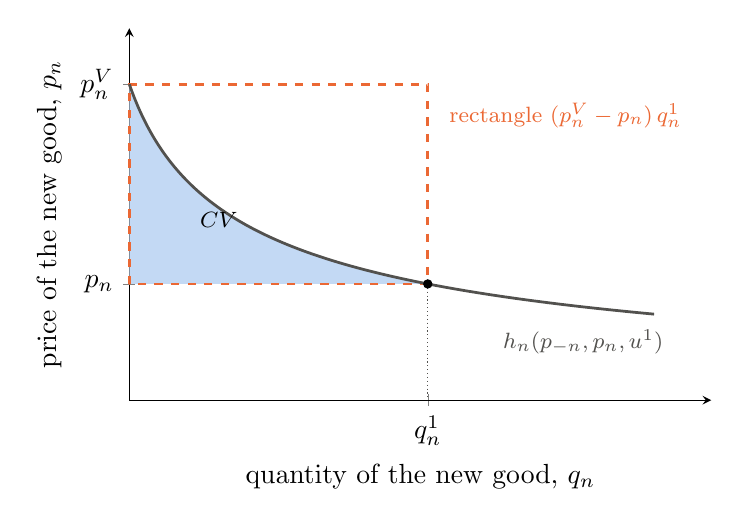
\begin{tikzpicture}
\begin{axis}[
  width=0.74\textwidth, height=0.52\textwidth,
  axis lines=left, xmin=0, xmax=1.95, ymin=0, ymax=3.2,
  xlabel={quantity of the new good, $q_n$}, ylabel={price of the new good, $p_n$},
  xtick={1}, xticklabels={$q_n^1$},
  ytick={1,2.71828}, yticklabels={$p_n$,$p_n^V$},
  every axis plot/.append style={line width=1pt},
  clip=false]
\addplot[draw=none, fill=c10p1blue!28, domain=1:2.71828, samples=80, variable=\t]
  ({(1-ln(\t))/\t},{\t}) -- (axis cs:0,2.71828) -- (axis cs:0,1) -- cycle;
\draw[dashed, c10p1orange, line width=1pt] (axis cs:0,1) rectangle (axis cs:1,2.71828);
\addplot[c10p1gray, domain=0.74:2.71828, samples=120, variable=\t] ({(1-ln(\t))/\t},{\t});
\draw[densely dotted, c10p1gray] (axis cs:1,1) -- (axis cs:1,0);
\fill (axis cs:1,1) circle (1.7pt);
\node[font=\footnotesize] at (axis cs:0.30,1.55) {$CV$};
\node[anchor=west, font=\footnotesize, text=c10p1orange] at (axis cs:1.04,2.45)
  {rectangle $(p_n^V - p_n)\,q_n^1$};
\node[anchor=west, font=\footnotesize, text=c10p1gray] at (axis cs:1.22,0.50)
  {$h_n(p_{-n},p_n,u^1)$};
\end{axis}
\end{tikzpicture}
\caption{The value of a new good. The curve is a compensated demand curve at the period-1 utility $u^1$. The
good sells at $p_n$, where the consumer buys $q_n^1$, and demand reaches zero at the virtual price $p_n^V$.
The shaded area is the compensating variation of \cref{prop:10-cv-newgood}. The dashed rectangle is the
Paasche bound of \cref{prop:10-index-bounds}. The curve drawn is $h_n = \frac{1 - \ln p_n}{p_n}$, so that
$p_n = q_n^1 = 1$ and $p_n^V = e$. The shaded area is $0.50$ and the rectangle is $1.72$.}
\label{fig:10-cv-area}
\end{figure}

\begin{remark}[Other prices, Marshallian surplus and Willig's approximation]\label{rem:10-willig}
If the prices of the other goods also change, from $p_{-n}^0$ to $p_{-n}^1$, the definition gives
$CV = e^R(p_{-n}^0,u^1) - e(p^1,u^1) = e\bigl(p_{-n}^0,p_n^V(p_{-n}^0,u^1),u^1\bigr) - y$. This is equation
(4) of \citet{Hausman1997} with all prices allowed to move, and \cref{sec:10-accounting} decomposes it. The
\emph{Marshallian surplus} of the new good is $CS = \int_{p_n}^{p_n^M}q_n(p_{-n},t,y)\,\dd t$. The argument
of \cref{prop:05-cv-ordering} applied on $[p_n,\infty)$ gives $EV \le CS \le CV$ for a normal good.
\citet{Willig1976} shows that the proportional gap $\frac{CV - CS}{CS}$ is approximately
$\frac{\bar\varepsilon_y\, CS}{2y}$ when the surplus is a small fraction of income, where $\bar\varepsilon_y$ is
the income elasticity of demand. His bounds replace $\bar\varepsilon_y$ by its smallest and largest values over the
price path. For a new good this path ends where the quantity reaches zero. If $\frac{\partial q_n}{\partial y}$
stays positive along the way, the income elasticity $\frac{\partial q_n}{\partial y}\frac{y}{q_n}$ grows without
bound, and the upper bound loses its force. \Cref{ex:10-linear-income} shows that the exact calculation is
easy in any case.

\citet[Section~7.4, pp.~184--188]{DeatonMuellbauer1980b} give a textbook account of these welfare measures. They
define both variations as differences of cost functions (their eqs.~4.1--4.2, p.~186). Our $CV$ is their
compensating variation for the move from $p^1$ back to $p^0$, the withdrawal of the good. They also explain why a
Marshallian area is not exact in general. It treats the marginal utility of income as constant, and that cannot
hold for all price changes (p.~185). For one good, the Hicksian and Marshallian demands coincide when utility is
quasi-linear in another good (Exercise~7.21, p.~189).
\end{remark}

\subsection{The cost-of-living index and the new-goods bias}\label{sec:10-col}

A cost-of-living index asks how much more, or less, income a consumer needs in period 1 to be as well off as
in period 0 \citep[p.~209]{Hausman1997}. \citet{Pollak1989} develops the theory.

\begin{definition}[Konüs cost-of-living index]\label{def:10-konus}
The \emph{cost-of-living index} between price vectors $p^0$ and $p^1$ at reference utility $u$ is
\begin{equation}\label{eq:10-konus}
  P(p^0,p^1,u) = \frac{e(p^1,u)}{e(p^0,u)}.
\end{equation}
\end{definition}

The index depends on the reference utility unless preferences are homothetic.
\citet[Section~7.1, pp.~170--173]{DeatonMuellbauer1980b} develop the index from the cost function. They show that
homotheticity is both necessary and sufficient for the index to be the same at every reference utility (p.~173).
With a new good the period-0
cost of reaching $u$ is $e^R(p_{-n}^0,u)$, which by \cref{lem:10-rothbarth}(c) equals
$e(p_{-n}^0,p_n^V,u)$. The period-0 price vector is therefore completed by the virtual price,
$p^0 = (p_{-n}^0,p_n^V(p_{-n}^0,u))$. With the period-1 reference and unchanged other prices,
\begin{equation}\label{eq:10-konus-newgood}
  P(p^0,p^1,u^1) = \frac{e(p_{-n},p_n,u^1)}{e(p_{-n},p_n^V,u^1)} = \frac{y}{y + CV} < 1 .
\end{equation}
The cost of living falls when a good is introduced. In the notation of \cref{lem:10-restricted}, the index is
$\frac{e(p,u^1)}{\tilde e(p,u^1,0)}$. Its reciprocal is the ratio of restricted to unrestricted cost, which
\citet[Exercise~7.16, p.~184]{DeatonMuellbauer1980b} propose as a measure of the cost of a ration.
\citet[p.~212]{Hausman1997} writes $y^*$ for
$e(p_{-n},p_n^V,u^1)$ and reports the reciprocal $\frac{y^*}{y}$, the cost of the period-1 standard of
living without the good relative to its cost with the good.

Statistical agencies compute \emph{matched-model} indexes. They compare the prices of goods sold in both
periods and add a new good to the sample only after it has been introduced. \citet[p.~210, n.~1]{Hausman1997}
notes that this procedure misses the gain at introduction, the welfare difference relative to a base period
in which the good was not sold. When the other prices do not change, every matched-model index equals one
between periods 0 and 1, whatever its formula. Comparing with \eqref{eq:10-konus-newgood},
\begin{equation}\label{eq:10-newgoods-bias}
  \frac{P^{MM}}{P(p^0,p^1,u^1)} - 1 = \frac{CV}{y},
\end{equation}
where $P^{MM} = 1$ is the matched-model index. The proportional overstatement of the price index equals the
value of the new good as a share of income. \citet[pp.~237--238]{Bresnahan1997} puts the point in terms of
timing. Official indexes link a new good in only after it has been sold for a while. They treat it as
irrelevant in its early stages, and the later the link, the larger the understatement of its value.

\subsection{Index-number bounds}\label{sec:10-bounds}

Index numbers built from observed prices and quantities bound the exact index. Let $q^0$ and $q^1$ be the
bundles bought in periods 0 and 1, with $q_n^0 = 0$ and $q_n^1 > 0$. Complete the period-0 prices with the
Hicksian virtual price at the period-1 utility, $p_n^0 = p_n^V(p_{-n},u^1)$. The \emph{Laspeyres} and
\emph{Paasche} indexes are
\begin{equation}\label{eq:10-LP}
  P_L = \frac{(p^1)^\top q^0}{(p^0)^\top q^0}, \qquad P_P = \frac{(p^1)^\top q^1}{(p^0)^\top q^1}.
\end{equation}
The Laspeyres index does not need $p_n^0$, because $q_n^0 = 0$. We write $w_n = \frac{p_nq_n^1}{y}$ for the
period-1 budget share of the new good.

\begin{proposition}[Index-number bounds for a new good]\label{prop:10-index-bounds}
Let Assumption~\ref{ass:10-prefs} hold, hold $p_{-n}$ and $y$ fixed, and suppose $p_n^V = p_n^V(p_{-n},u^1)$ is finite.
\begin{enumerate}[label=(\alph*)]
  \item The Laspeyres index records no change: $P_L = 1$.
  \item The Paasche index is $P_P = \frac{y}{y + (p_n^V - p_n)q_n^1}$.
  \item The exact index lies between them, $P_P \le P(p^0,p^1,u^1) \le P_L$. Equivalently,
  \begin{equation}\label{eq:10-cv-bounds}
    0 \le CV \le (p_n^V - p_n)\,q_n^1 .
  \end{equation}
  \item In share form, $\frac{CV}{y} \le w_n\Bigl(\frac{p_n^V}{p_n} - 1\Bigr)$.
\end{enumerate}
\end{proposition}

\begin{proof}
(a) Since $q_n^0 = 0$ and the other prices are unchanged,
$(p^1)^\top q^0 = \sum_{j\neq n}p_jq_j^0 = (p^0)^\top q^0$.

(b) The numerator is period-1 spending, $(p^1)^\top q^1 = y$. The denominator is
\begin{equation*}
  (p^0)^\top q^1 = \sum_{j\neq n}p_jq_j^1 + p_n^Vq_n^1 = y - p_nq_n^1 + p_n^Vq_n^1 = y + (p_n^V - p_n)q_n^1 .
\end{equation*}

(c) By \cref{prop:10-cv-newgood}, $CV = \int_{p_n}^{p_n^V}h_n(p_{-n},t,u^1)\,\dd t$. Hicksian demand is
nonnegative and nonincreasing in its own price, and $h_n(p_{-n},p_n,u^1) = q_n^1$ by \eqref{eq:10-duality}.
Hence, for every $t \in [p_n,p_n^V]$,
\begin{equation*}
  0 \le h_n(p_{-n},t,u^1) \le q_n^1 .
\end{equation*}
Integrating over $[p_n,p_n^V]$ gives \eqref{eq:10-cv-bounds}. Substituting the bounds into
\eqref{eq:10-konus-newgood} gives $P_P \le P \le 1 = P_L$.

(d) Divide \eqref{eq:10-cv-bounds} by $y$ and write $(p_n^V - p_n)q_n^1 = p_nq_n^1\bigl(\frac{p_n^V}{p_n} - 1\bigr)$.
\end{proof}

The Laspeyres bound is the matched-model index of \cref{sec:10-col}, and it says nothing. The Paasche bound is
the rectangle in \cref{fig:10-cv-area}. \citet[p.~212]{Hausman1997} describes the index-number approach of
Hicks and Rothbarth as measuring the change in real income by the ratio $\frac{p_n^Vq_n}{p_nq_n}$. The ratio
compares the value of the new good's purchases at the virtual price with their value at the actual price. Its
numerator minus its denominator is the rectangle. Hausman calls the approach approximately correct but notes
that it ignores the income compensation needed to stay on the indifference curve. \Cref{prop:10-index-bounds}
adds that the rectangle is an upper bound. Part (d) is the logic behind the rule of thumb that
\cref{sec:10-hausman} examines: the new good's share times the proportional gap between its virtual and
actual prices.

\begin{corollary}[Linear, convex and concave demand]\label{cor:10-half}
Under the conditions of \cref{prop:10-index-bounds}, if $h_n(p_{-n},t,u^1)$ is linear in $t$ on
$[p_n,p_n^V]$, then $CV = \frac{1}{2}(p_n^V - p_n)q_n^1$. If it is convex on that interval,
$CV \le \frac{1}{2}(p_n^V - p_n)q_n^1$. If it is concave, $CV \ge \frac{1}{2}(p_n^V - p_n)q_n^1$.
\end{corollary}

\begin{proof}
The chord joining $(p_n,q_n^1)$ and $(p_n^V,0)$ is $\ell(t) = q_n^1\frac{p_n^V - t}{p_n^V - p_n}$, and its
integral over $[p_n,p_n^V]$ is the triangle $\frac{1}{2}(p_n^V - p_n)q_n^1$. A linear function equals its
chord. A convex function lies below its chord between the two endpoints, and a concave function lies above
it. Integrating gives the three claims.
\end{proof}

\begin{remark}[The Konüs inequalities and a second-order view]\label{rem:10-konus}
Part (c) of \cref{prop:10-index-bounds} is a case of two inequalities due to \citet{Konus1939}.
\citet[Section~7.1, eqs.~1.3--1.4, p.~172]{DeatonMuellbauer1980b} give the standard proof. The bundle $q^1$ is one
way to reach $u^1$ at prices $p^0$, so it costs at least the minimum, $(p^0)^\top q^1 \ge e(p^0,u^1)$. Since
$(p^1)^\top q^1 = e(p^1,u^1)$,
\begin{equation*}
  P_P = \frac{(p^1)^\top q^1}{(p^0)^\top q^1} \le \frac{e(p^1,u^1)}{e(p^0,u^1)} = P(p^0,p^1,u^1).
\end{equation*}
The same argument with $q^0$ at prices $p^1$ gives $P_L \ge P(p^0,p^1,u^0)$. In general the two bounds apply at
different reference utilities, so the true index need not lie between them (p.~172). With a new good the
Laspeyres index equals one. \Cref{lem:10-rothbarth}(a) puts the true index below one at every reference utility.
This is why part (c) can bracket the index at the single reference $u^1$.

Deaton and Muellbauer also show that the Laspeyres index is a first-order approximation to the true index
(eqs.~1.6--1.7, p.~174). For a new good the first-order term is zero. Expand $t \mapsto e(p_{-n},t,u^1)$ to second
order around $p_n^V$. By Shephard's lemma its first derivative there is $h_n(p_{-n},p_n^V,u^1) = 0$, so
\begin{equation*}
  CV = e\bigl(p_{-n},p_n^V,u^1\bigr) - e\bigl(p_{-n},p_n,u^1\bigr)
  \approx -\frac{1}{2}\,\frac{\partial h_n}{\partial p_n}\,\bigl(p_n^V - p_n\bigr)^2 .
\end{equation*}
The value of a new good is thus a pure substitution effect, which an index with fixed base weights cannot capture.
If $h_n$ is linear on $[p_n,p_n^V]$, the expansion is exact. Substituting
$-\frac{\partial h_n}{\partial p_n} = \frac{q_n^1}{p_n^V - p_n}$ then gives $CV = \frac{1}{2}(p_n^V - p_n)q_n^1$, as
in \cref{cor:10-half}. Their first-order approximation to a compensating variation, the reference quantities times
the price changes (eq.~4.3, p.~187), is here the Paasche rectangle $(p_n^V - p_n)q_n^1$.
\end{remark}

\subsection{Separability: which demand curves are needed}\label{sec:10-separability}

Applying \cref{prop:10-cv-newgood} seems to require the whole expenditure function. \citet[p.~213,
n.~7]{Hausman1997} argues that under the usual separability assumptions only the demand curve for the new
good must be estimated. The next result makes the claim precise for homothetic separability, the first case
of Gorman's two-stage budgeting theorem (\cref{prop:05-first-stage}).

\begin{assumption}[Homothetic separability]\label{ass:10-hsep}
The goods are split into a group $N$ that contains good $n$ and the remaining goods. Utility is
$U(q) = F(q_{-N},\phi(q_N))$, where $F$ is strictly increasing in its last argument and the subutility $\phi$
is continuous, increasing, quasi-concave and homogeneous of degree one.
\end{assumption}

Let $P_N(p_N) = \min\{p_N^\top q_N : \phi(q_N) \ge 1\}$ be the unit cost of the subutility. It is the exact
price index of the group. Let $w_{n|N}(p_N) = \frac{\partial\ln P_N}{\partial\ln p_n}$ be the within-group
budget share of good $n$, which depends only on the prices of the group.

\begin{proposition}[New goods in a separable group]\label{prop:10-separable}
Under Assumptions~\ref{ass:10-prefs} and~\ref{ass:10-hsep}, the following hold.
\begin{enumerate}[label=(\alph*)]
  \item The expenditure function has the form $e(p,u) = E(p_{-N},P_N(p_N),u)$, where $E$ is the expenditure
  function for the goods outside $N$ and a composite good $Q_N = \phi(q_N)$ with price $P_N$.
  \item Fix $p_{-n}$ and $u$. Suppose the Hicksian demand for the composite is positive at every $p_n$ below the
  smallest $p_n$ at which $\frac{\partial P_N}{\partial p_n} = 0$. Then the Hicksian virtual price of good $n$ is
  that smallest $p_n$, and it depends only on the other prices of group $N$.
  \item Let $P_N^R = P_N(p_{N\setminus n},p_n^V)$ be the group index without the new good. Then
  \begin{equation}\label{eq:10-sep-index}
    \ln\frac{P_N^R}{P_N} = \int_{p_n}^{p_n^V}\frac{w_{n|N}(p_{N\setminus n},t)}{t}\,\dd t,
  \end{equation}
  \begin{equation}\label{eq:10-sep-cv}
    CV = E(p_{-N},P_N^R,u^1) - E(p_{-N},P_N,u^1) = \int_{P_N}^{P_N^R}H_N(p_{-N},\tau,u^1)\,\dd\tau,
  \end{equation}
  where $H_N = \frac{\partial E}{\partial P_N}$ is the Hicksian demand for the composite good.
\end{enumerate}
\end{proposition}

\begin{proof}
(a) Fix $u$ and minimize cost in two steps. Given a level $Q_N$ of the composite, the cheapest bundle with
$\phi(q_N) \ge Q_N$ costs $P_N(p_N)\,Q_N$, because $\phi$ is homogeneous of degree one. The consumer then
chooses $q_{-N}$ and $Q_N$ to minimize $p_{-N}^\top q_{-N} + P_NQ_N$ subject to $F(q_{-N},Q_N) \ge u$. The
value of this problem is $E(p_{-N},P_N,u)$.

(b) By Shephard's lemma and the chain rule,
\begin{equation*}
  h_n(p,u) = \frac{\partial E}{\partial P_N}\cdot\frac{\partial P_N}{\partial p_n} = H_N(p_{-N},P_N,u)\,\frac{\partial P_N}{\partial p_n}.
\end{equation*}
By hypothesis $H_N > 0$ below the first zero of $\frac{\partial P_N}{\partial p_n}$, so $h_n > 0$ there. At that
zero $h_n = 0$. The virtual price is therefore the first zero of $\frac{\partial P_N}{\partial p_n}$, a condition on
$p_N$ alone.

(c) Shephard's lemma applied to the unit cost gives $\frac{\partial\ln P_N}{\partial p_n} = \frac{w_{n|N}}{p_n}$.
Integrating in $p_n$ from $p_n$ to $p_n^V$ with the other group prices fixed gives \eqref{eq:10-sep-index}. For
\eqref{eq:10-sep-cv}, \eqref{eq:10-cv-e} and part (a) give
$CV = E(p_{-N},P_N^R,u^1) - E(p_{-N},P_N,u^1)$. Shephard's lemma for $E$ and the fundamental theorem of
calculus give the integral.
\end{proof}

The proposition splits the calculation into two stages. The change in the group index needs only the new good's
within-group share as a function of its own price, at the observed prices of the other goods in the group. In
that sense Hausman's claim holds. Part (b) needs its positivity condition. If the whole group can leave consumption,
$H_N$ can reach zero before $\frac{\partial P_N}{\partial p_n}$ does. The Hicksian virtual price is then the lower
price at which $H_N$ vanishes, and it can depend on $u$ and on prices outside the group. Part (c) still holds if we
evaluate $P_N^R$ at the first zero of $\frac{\partial P_N}{\partial p_n}$, because $E$ does not change with $P_N$
once $H_N = 0$. Converting the group index change into money needs the demand for the group
as a whole. If compensated group spending $X_N$ stays roughly constant over the relevant range, then
$CV \approx X_N\ln\frac{P_N^R}{P_N}$. The index used at the upper stage must be the exact group index with the
virtual price inserted for the period before the introduction. A Stone or matched-model index of the old
goods records no change. \citet[p.~221]{Hausman1997} rejects homotheticity of brand choice in his cereal
data. For groups that are not homothetic, two-stage budgeting holds only approximately or under the
generalized Gorman polar form of \cref{def:05-ggpf}. \citet{Gorman1959} gives the conditions.

\citet[Section~5.2, pp.~128--133]{DeatonMuellbauer1980b} give a textbook account of these conditions. The upper
stage allocates income across groups $G$ through group cost functions $c_G(u_G,p_G)$, subject to
$\sum_Gc_G(u_G,p_G) = y$ (their eqs.~2.11--2.14, p.~130). Gorman's first case has group cost functions of the form
$\theta_G(u_G)\,b_G(p_G)$, which is Assumption~\ref{ass:10-hsep} (eq.~2.15, p.~130). His second case is the generalized
polar form with utility additive across groups (eqs.~2.16--2.17, pp.~130--131). Weak separability also restricts substitution
across groups. For good $n$ in group $N$ and good $j$ in another group $H$, the compensated cross-price effect is
\begin{equation*}
  \frac{\partial h_n}{\partial p_j} = m_{NH}\,\frac{\partial q_n}{\partial y}\,\frac{\partial q_j}{\partial y},
\end{equation*}
where the scalar $m_{NH}$ depends only on the two groups (eq.~2.8, p.~128). A new good therefore reaches the
demand for a good in another group only through the expenditure allocated to that group.

\subsection{The CES variety-adjusted price index}\label{sec:10-feenstra}

Constant elasticity of substitution (CES) preferences give the best known correction of a price index for new
varieties \citep{Feenstra1994}. Let $\mathcal{I}_t$ be the set of varieties available in period $t$, with
taste parameters $a_j > 0$. The CES unit expenditure function is
\begin{equation}\label{eq:10-ces-unit}
  c(p;\mathcal{I}) = \Bigl(\sum_{j\in\mathcal{I}}a_jp_j^{1-\eta}\Bigr)^{\frac{1}{1-\eta}}, \qquad \eta > 1,
\end{equation}
and preferences are homothetic, so $e(p,u) = c(p;\mathcal{I})\,u$. Here $\eta$ is the elasticity of
substitution. \citet{Hausman1997} writes the CES utility function with a parameter $\rho$, and
$\eta = \frac{1}{1-\rho}$. \Cref{ch:aids} writes $\sigma$ for $\eta$, a symbol this chapter keeps for the
nesting parameter.

Shephard's lemma gives the expenditure shares. Differentiating \eqref{eq:10-ces-unit},
\begin{equation*}
  \frac{\partial c}{\partial p_j} = \frac{1}{1-\eta}\Bigl(\sum_k a_kp_k^{1-\eta}\Bigr)^{\frac{1}{1-\eta}-1}(1-\eta)a_jp_j^{-\eta}
  = c^{\eta}a_jp_j^{-\eta}.
\end{equation*}
The share of variety $j$ is therefore
\begin{equation}\label{eq:10-ces-share}
  w_j = \frac{p_j}{c}\frac{\partial c}{\partial p_j} = a_j\Bigl(\frac{p_j}{c}\Bigr)^{1-\eta}
  = \frac{a_jp_j^{1-\eta}}{\sum_{k\in\mathcal{I}}a_kp_k^{1-\eta}} .
\end{equation}

The first step handles a fixed set of varieties. For two positive numbers let
$\mathcal{L}(a,b) = \frac{a - b}{\ln a - \ln b}$ if $a \neq b$ and $\mathcal{L}(a,a) = a$. This is the
\emph{logarithmic mean}.

\begin{lemma}[Sato-Vartia index, \citealp{Sato1976,Vartia1976}]\label{lem:10-sato-vartia}
Let $\mathcal{I}$ be a set of varieties available in periods $t-1$ and $t$, with the same $a_j$ in both
periods. Let $\tilde w_{jt}$ be the share of variety $j$ in period-$t$ spending on $\mathcal{I}$. Then
\begin{equation}\label{eq:10-sv}
  \frac{c(p_t;\mathcal{I})}{c(p_{t-1};\mathcal{I})} = P^{SV}_{\mathcal{I}}
  \equiv \prod_{j\in\mathcal{I}}\Bigl(\frac{p_{jt}}{p_{j,t-1}}\Bigr)^{\omega_j}, \qquad
  \omega_j = \frac{\mathcal{L}(\tilde w_{jt},\tilde w_{j,t-1})}{\sum_{k\in\mathcal{I}}\mathcal{L}(\tilde w_{kt},\tilde w_{k,t-1})}.
\end{equation}
\end{lemma}

\begin{proof}
Write $c_t = c(p_t;\mathcal{I})$. Taking logs of \eqref{eq:10-ces-share} for the set $\mathcal{I}$ gives
$\ln\tilde w_{jt} = \ln a_j + (1-\eta)(\ln p_{jt} - \ln c_t)$. Differencing over time removes $\ln a_j$:
\begin{equation*}
  \Delta\ln\tilde w_j = (1-\eta)\bigl(\Delta\ln p_j - \Delta\ln c\bigr), \qquad j \in \mathcal{I}.
\end{equation*}
Solving for the change in the unit cost gives, for every $j$,
\begin{equation*}
  \Delta\ln c = \Delta\ln p_j - \frac{1}{1-\eta}\Delta\ln\tilde w_j .
\end{equation*}
Multiply by $\omega_j$ and sum over $j$. The weights sum to one, so
\begin{equation*}
  \Delta\ln c = \sum_{j\in\mathcal{I}}\omega_j\Delta\ln p_j - \frac{1}{1-\eta}\sum_{j\in\mathcal{I}}\omega_j\Delta\ln\tilde w_j .
\end{equation*}
By the definition of the logarithmic mean, $\mathcal{L}(\tilde w_{jt},\tilde w_{j,t-1})\Delta\ln\tilde w_j =
\tilde w_{jt} - \tilde w_{j,t-1}$. The shares sum to one in each period, so
$\sum_j\omega_j\Delta\ln\tilde w_j$ is proportional to $\sum_j(\tilde w_{jt} - \tilde w_{j,t-1}) = 0$. The
second term vanishes, and exponentiating gives \eqref{eq:10-sv}.
\end{proof}

The Sato-Vartia index uses only observed prices and quantities, and it is exact for CES preferences without
knowledge of $\eta$. New varieties enter through a second factor. Let $\mathcal{I} \subseteq
\mathcal{I}_{t-1}\cap\mathcal{I}_t$ be a nonempty set of varieties sold in both periods, with unchanged $a_j$.
Let $\lambda_t$ be the share of period-$t$ spending that goes to $\mathcal{I}$, and $\lambda_{t-1}$ the
corresponding share in period $t-1$:
\begin{equation*}
  \lambda_t = \frac{\sum_{j\in\mathcal{I}}p_{jt}q_{jt}}{\sum_{j\in\mathcal{I}_t}p_{jt}q_{jt}}, \qquad
  \lambda_{t-1} = \frac{\sum_{j\in\mathcal{I}}p_{j,t-1}q_{j,t-1}}{\sum_{j\in\mathcal{I}_{t-1}}p_{j,t-1}q_{j,t-1}}.
\end{equation*}

\begin{proposition}[CES index with changing varieties, \citealp{Feenstra1994}]\label{prop:10-feenstra}
Under CES preferences \eqref{eq:10-ces-unit},
\begin{equation}\label{eq:10-feenstra}
  \frac{c(p_t;\mathcal{I}_t)}{c(p_{t-1};\mathcal{I}_{t-1})}
  = P^{SV}_{\mathcal{I}}\,\Bigl(\frac{\lambda_t}{\lambda_{t-1}}\Bigr)^{\frac{1}{\eta-1}} .
\end{equation}
\end{proposition}

\begin{proof}
By \eqref{eq:10-ces-unit}, $\sum_{j\in\mathcal{I}}a_jp_{jt}^{1-\eta} = c(p_t;\mathcal{I})^{1-\eta}$ and
$\sum_{j\in\mathcal{I}_t}a_jp_{jt}^{1-\eta} = c(p_t;\mathcal{I}_t)^{1-\eta}$. Summing \eqref{eq:10-ces-share}
over $j \in \mathcal{I}$ gives the share of the common varieties,
\begin{equation*}
  \lambda_t = \frac{c(p_t;\mathcal{I})^{1-\eta}}{c(p_t;\mathcal{I}_t)^{1-\eta}} .
\end{equation*}
Solving for the full unit cost,
\begin{equation*}
  c(p_t;\mathcal{I}_t) = c(p_t;\mathcal{I})\,\lambda_t^{-\frac{1}{1-\eta}} = c(p_t;\mathcal{I})\,\lambda_t^{\frac{1}{\eta-1}} .
\end{equation*}
The same steps hold in period $t-1$. Taking the ratio of the two periods,
\begin{equation*}
  \frac{c(p_t;\mathcal{I}_t)}{c(p_{t-1};\mathcal{I}_{t-1})}
  = \frac{c(p_t;\mathcal{I})}{c(p_{t-1};\mathcal{I})}\Bigl(\frac{\lambda_t}{\lambda_{t-1}}\Bigr)^{\frac{1}{\eta-1}} .
\end{equation*}
\Cref{lem:10-sato-vartia} replaces the first ratio by $P^{SV}_{\mathcal{I}}$.
\end{proof}

A matched-model index computed on the common varieties is $P^{SV}_{\mathcal{I}}$. The second factor is the
correction for changing variety. When new varieties take a larger share of spending than the varieties that
disappear, $\lambda_t < \lambda_{t-1}$, and the correction lowers the index. The correction needs one
parameter, $\eta$. A low elasticity of substitution means a large correction, because the new varieties are
then poor substitutes for the old ones.

\begin{corollary}[One new variety]\label{cor:10-ces-newgood}
Suppose $\mathcal{I}_t = \mathcal{I}_{t-1}\cup\{n\}$, the other prices do not change, and the new variety
takes the share $w_n$ of period-$t$ spending. Then
\begin{equation}\label{eq:10-ces-newgood}
  \frac{c(p_t;\mathcal{I}_t)}{c(p_{t-1};\mathcal{I}_{t-1})} = (1 - w_n)^{\frac{1}{\eta-1}}, \qquad
  \frac{CV}{y} = (1 - w_n)^{-\frac{1}{\eta-1}} - 1, \qquad
  \frac{EV}{y} = 1 - (1 - w_n)^{\frac{1}{\eta-1}} .
\end{equation}
For small $w_n$ both measures are close to $\frac{w_n}{\eta - 1}$.
\end{corollary}

\begin{proof}
Take $\mathcal{I} = \mathcal{I}_{t-1}$. Unchanged prices give $P^{SV}_{\mathcal{I}} = 1$, and
$\lambda_{t-1} = 1$ and $\lambda_t = 1 - w_n$. \Cref{eq:10-feenstra} gives the first formula. Write
$c_0 = c(p_{t-1};\mathcal{I}_{t-1})$ and $c_1 = c(p_t;\mathcal{I}_t)$. Period-$t$ income is $y = c_1u^1$, and
the consumer would need $c_0u^1$ to reach $u^1$ without the new variety. Hence
$\frac{CV}{y} = \frac{c_0u^1 - c_1u^1}{c_1u^1} = \frac{c_0}{c_1} - 1$. Similarly, $y = c_0u^0$ and
$\frac{EV}{y} = \frac{c_0u^0 - c_1u^0}{c_0u^0} = 1 - \frac{c_1}{c_0}$. The approximation is the first-order
expansion of $(1 - w_n)^{\pm\frac{1}{\eta-1}}$ around $w_n = 0$.
\end{proof}

The formula for $CV$ is the removal formula of \cref{prop:05-variety}(a) read in reverse. Two features stand
out. First, CES demand is positive at every price, so the virtual price of the new variety is infinite. The
gain is nonetheless finite, because the CES demand curve approaches the price axis fast enough. Second, the
gain depends only on the new variety's share and on $\eta$. Nothing in the formula measures how close the new
variety is to particular old ones. \citet[p.~230]{Hausman1997} draws the conclusion that the CES, like the
logit, ``will tend to overvalue variety'' because it treats all goods symmetrically.

\begin{remark}[CES and logit]\label{rem:10-ces-logit}
The parallel with the logit model is exact. \Cref{sec:10-charspace} shows that adding a product with
post-introduction share $s_n$ to a logit market raises expected consumer surplus by
$-\frac{1}{\alpha}\ln(1 - s_n)$ per consumer. This is again a function of one share and one parameter
\citep{SmallRosen1981,McFadden1981}. \citet{AndersonDePalmaThisse1992} explain why, and
\citet[n.~29]{Hausman1997} cites them. Suppose each consumer buys one variety and spends all income on it,
with conditional indirect utility $\ln y - \ln p_j + \theta_j + \mu\epsilon_{ij}$ and type-I extreme value
$\epsilon_{ij}$. The logit choice probability is
$\Pr_j = \frac{e^{\frac{\theta_j}{\mu}}p_j^{-\frac{1}{\mu}}}{\sum_ke^{\frac{\theta_k}{\mu}}p_k^{-\frac{1}{\mu}}}$.
Each buyer of $j$ purchases $\frac{y}{p_j}$ units, so expected demand per consumer is
\begin{equation*}
  \frac{y\Pr_j}{p_j} = \frac{y\,e^{\frac{\theta_j}{\mu}}p_j^{-\frac{1}{\mu}-1}}{\sum_ke^{\frac{\theta_k}{\mu}}p_k^{-\frac{1}{\mu}}} .
\end{equation*}
This is the CES demand $\frac{y\,a_jp_j^{-\eta}}{\sum_ka_kp_k^{1-\eta}}$ implied by \eqref{eq:10-ces-share}, with
$\eta = 1 + \frac{1}{\mu}$ and $a_j = e^{\frac{\theta_j}{\mu}}$. Expected maximum utility is
$\ln y + \mu\ln\sum_ka_kp_k^{-\frac{1}{\mu}}$ plus a constant. Since $\mu(1-\eta) = -1$, this equals
$\ln y - \ln c(p;\mathcal{I})$ plus a constant, the CES indirect utility in logs. In both models each variety
carries its own taste shock, and the value of variety is built into the functional form.
\end{remark}

As an illustration, take two numbers from \citet{Hausman1997}. His reported CES elasticity is $\eta = 2.13$
(p.~231). His printed $\hat\rho = 0.580$ would imply 2.38, an inconsistency that \cref{sec:10-hausman-ces}
discusses. In addition, Apple-Cinnamon Cheerios had a 6.19 percent share of the family segment of ready-to-eat cereal in 1992
(Table 5.2). Treat the segment as a CES group. \Cref{cor:10-ces-newgood} then gives our computation
$(1 - 0.0619)^{\frac{1}{1.13}} = 0.945$.
The introduction lowers the segment's cost of living by 5.5 percent, and the compensating variation is 5.8
percent of segment spending. Hausman reports that his own CES specification gives a consumer surplus about
three times as large as his preferred estimate (p.~231). \Cref{sec:10-hausman} returns to the comparison.

\section{Functional form, extrapolation and bounds}\label{sec:10-functional}

The exact measures of \cref{sec:10-virtual} integrate the compensated demand curve from the observed price to
the virtual price. This section asks how much of that integral the data can deliver. We show that the answer
depends on the shape assumed beyond the data, and we compare three standard shapes. We then explain how to
recover the exact measure from an estimated Marshallian demand curve and derive a lower bound that needs only
convexity.

\subsection{The extrapolation problem}\label{sec:10-extrapolation}

Prices in a sample vary within a band around the observed price. In Hausman's cereal data the variation is on
the order of 50 percent, and prices as high as the estimated virtual price are never observed
\citep[p.~228]{Hausman1997}. His virtual price is about twice the actual price. The part of the area in
\cref{fig:10-cv-area} that lies above the highest observed price is then pinned down by the functional form
alone.

\citet[Section 1]{BerryPakes2007} make the general point. We rarely see demand for a new product at prices high
enough to estimate the reservation prices of many consumers without parametric assumptions. A demand system in
product space obtains the gains of inframarginal buyers by extending the curve estimated at low prices into a
higher price range. That extension can be very sensitive to the model. A demand system in characteristics
space also uses the price variation of products with similar characteristics. It therefore uses more
information, but similar problems arise. \Cref{sec:10-charspace} develops the characteristics approach.

The problem can be stated as a question of identification. Suppose the data reveal $h_n(p_{-n},t,u^1)$ for
$t \in [p_n,\bar p]$, with $\bar p$ the highest observed price and $h_n(p_{-n},\bar p,u^1) > 0$. Split the
compensating variation at $\bar p$:
\begin{equation}\label{eq:10-cv-split}
  CV = \underbrace{\int_{p_n}^{\bar p}h_n(p_{-n},t,u^1)\,\dd t}_{\text{supported by data}}
  + \underbrace{\int_{\bar p}^{p_n^V}h_n(p_{-n},t,u^1)\,\dd t}_{\text{extrapolated}} .
\end{equation}
Any nonincreasing extension of the demand curve beyond $\bar p$ agrees with the data. A curve that stays flat
at $h_n(p_{-n},\bar p,u^1)$ over a long interval before dropping to zero makes the second term as large as we
like. Without restrictions on shape, the data identify only the lower bound given by the first term. Bounds
that are more useful need restrictions, and point estimates need a functional form.

\subsection{Three canonical shapes}\label{sec:10-shapes}

Fix an observed point $(p,q)$ on the demand curve for good $n$. Let $\varepsilon = -\frac{p\,q'(p)}{q} > 0$
be the elasticity of demand at that point, written as a positive number as in the rest of the book. We compare
three demand curves that share the point and the slope. To keep the formulas transparent we integrate the
demand curve as drawn, and write $CS$ for the area.

\casehead{Linear demand}
Let $q(t) = a - bt$. Matching the slope gives $b = \frac{\varepsilon q}{p}$, and matching the point gives
$a = q + bp$. Demand reaches zero at
\begin{equation*}
  p^V = \frac{a}{b} = p + \frac{q}{b} = p\Bigl(1 + \frac{1}{\varepsilon}\Bigr).
\end{equation*}
The area is a triangle with height $p^V - p = \frac{q}{b}$ and base $q$:
\begin{equation*}
  CS = \int_p^{\frac{a}{b}}(a - bt)\,\dd t = \frac{(a - bp)^2}{2b} = \frac{q^2}{2b} = \frac{pq}{2\varepsilon}.
\end{equation*}

\casehead{AIDS demand with $\beta_n = 0$}
In the almost ideal demand system the budget share of good $n$ is linear in log prices. With $\beta_n = 0$ and
the other prices fixed, $w(t) = w + \gamma\ln\frac{t}{p}$, where $w$ is the observed share and $\gamma =
\gamma_{nn}$ (\cref{sec:05-aids}). Quantity is $q(t) = \frac{y\,w(t)}{t}$. The budget share does not depend on income, but quantity
has income elasticity one. Since $\ln q = \ln y + \ln w(t) -
\ln t$, the elasticity at $p$ is $\varepsilon = 1 - \frac{\gamma}{w}$. Hence $\gamma = -w(\varepsilon - 1)$,
which is negative when $\varepsilon > 1$. The share reaches zero where $\ln\frac{p^V}{p} = \frac{w}{-\gamma}$,
so
\begin{equation*}
  p^V = p\,\exp\Bigl(\frac{1}{\varepsilon - 1}\Bigr).
\end{equation*}
Substituting $x = \ln\frac{t}{p}$ and writing $x^V = \ln\frac{p^V}{p} = \frac{w}{-\gamma}$, the area is
\begin{equation*}
  CS = \int_p^{p^V}\frac{y\,w(t)}{t}\,\dd t = y\int_0^{x^V}(w + \gamma x)\,\dd x
  = y\Bigl(w\,x^V + \frac{\gamma\,(x^V)^2}{2}\Bigr) = \frac{y\,w^2}{2(-\gamma)} = \frac{pq}{2(\varepsilon - 1)}.
\end{equation*}
The last step uses $yw = pq$ and $-\gamma = w(\varepsilon - 1)$. With $\beta_n = 0$ the area also gives the
exact measure through $\ln(1 + \frac{CV}{y}) = \frac{CS}{y}$, which is \cref{prop:05-variety}(c).

\casehead{Constant-elasticity demand}
Let $q(t) = At^{-\varepsilon}$ with $A = qp^{\varepsilon}$. Demand is positive at every price, so $p^V = \infty$.
For $\varepsilon > 1$,
\begin{equation*}
  CS = \int_p^{\infty}At^{-\varepsilon}\,\dd t = \frac{Ap^{1-\varepsilon}}{\varepsilon - 1} = \frac{pq}{\varepsilon - 1}.
\end{equation*}
For $\varepsilon \le 1$ the integral diverges.

\Cref{tab:10-shapes} and \cref{fig:10-extrapolation} collect the three cases. Three lessons follow. First,
curves that agree on the level and slope of demand at the observed price give very different values. At
$\varepsilon = 2$ the constant-elasticity value is four times the linear one. Second, an infinite virtual price
does not imply an infinite gain. Third, both the AIDS and the constant-elasticity values explode as
$\varepsilon$ approaches one, while the linear value stays finite. The ratio of the constant-elasticity value
to the AIDS value is two at every elasticity. \citet[p.~231]{Hausman1997} finds a ratio of about three
between his CES and AIDS estimates.

\begin{table}[htbp]
\centering
\caption{Three demand curves through the same point}\label{tab:10-shapes}
\begin{threeparttable}
\begin{tabular}{@{}lcccc@{}}
\toprule
 & \multicolumn{2}{c}{General point $(p,q)$, elasticity $\varepsilon$} & \multicolumn{2}{c}{$p = q = 1$, $\varepsilon = 2$} \\
\cmidrule(lr){2-3}\cmidrule(lr){4-5}
Demand curve & Virtual price & Area $CS$ & Virtual price & Area $CS$ \\
\midrule
Linear & $p\bigl(1 + \frac{1}{\varepsilon}\bigr)$ & $\frac{pq}{2\varepsilon}$ & 1.50 & 0.25 \\[4pt]
AIDS with $\beta_n = 0$ & $p\exp\bigl(\frac{1}{\varepsilon - 1}\bigr)$ & $\frac{pq}{2(\varepsilon - 1)}$ & 2.72 & 0.50 \\[4pt]
Constant elasticity & $\infty$ & $\frac{pq}{\varepsilon - 1}$ & $\infty$ & 1.00 \\
\bottomrule
\end{tabular}
\begin{tablenotes}[flushleft]\footnotesize
\item Notes: Each curve passes through the observed point $(p,q)$ with own-price elasticity $\varepsilon > 1$,
written as a positive number. The area is the integral of the demand curve from $p$ to the virtual price. The
AIDS and constant-elasticity formulas require $\varepsilon > 1$. Derivations are in \cref{sec:10-shapes}, and
the numbers come from \texttt{figures/ch10/src/part1\_checks.py}.
\end{tablenotes}
\end{threeparttable}
\end{table}

\begin{figure}[htbp]
\centering
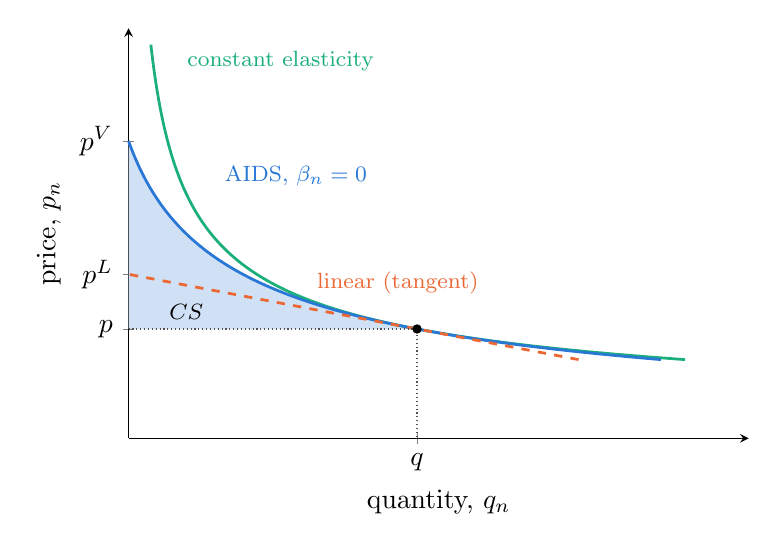
\begin{tikzpicture}
\begin{axis}[
  width=0.78\textwidth, height=0.56\textwidth,
  axis lines=left, xmin=0, xmax=2.15, ymin=0, ymax=3.75,
  xlabel={quantity, $q_n$}, ylabel={price, $p_n$},
  xtick={1}, xticklabels={$q$},
  ytick={1,1.5,2.71828}, yticklabels={$p$,$p^L$,$p^V$},
  every axis plot/.append style={line width=1pt},
  clip=false]
\addplot[draw=none, fill=c10p1blue!22, domain=1:2.71828, samples=80, variable=\t]
  ({(1-ln(\t))/\t},{\t}) -- (axis cs:0,2.71828) -- (axis cs:0,1) -- cycle;
\addplot[c10p1aqua, domain=0.72:3.6, samples=120, variable=\t] ({1/(\t*\t)},{\t});
\addplot[c10p1blue, domain=0.72:2.71828, samples=120, variable=\t] ({(1-ln(\t))/\t},{\t});
\addplot[c10p1orange, dashed, domain=0.72:1.5, samples=2, variable=\t] ({3-2*\t},{\t});
\draw[densely dotted, c10p1gray] (axis cs:0,1) -- (axis cs:1,1) -- (axis cs:1,0);
\fill (axis cs:1,1) circle (1.7pt);
\node[anchor=west, font=\footnotesize, text=c10p1aqua] at (axis cs:0.17,3.45) {constant elasticity};
\node[anchor=west, font=\footnotesize, text=c10p1blue] at (axis cs:0.30,2.40) {AIDS, $\beta_n = 0$};
\node[anchor=west, font=\footnotesize, text=c10p1orange] at (axis cs:0.62,1.42) {linear (tangent)};
\node[font=\footnotesize] at (axis cs:0.20,1.16) {$CS$};
\end{axis}
\end{tikzpicture}
\caption{Extrapolating demand beyond the data. All three curves pass through the observed point $(p,q) = (1,1)$
with own-price elasticity 2. The linear curve is the tangent at the observed point and reaches zero at
$p^L = 1.5$. The AIDS curve with $\beta_n = 0$ is convex and reaches zero at $p^V = e \approx 2.72$. The
constant-elasticity curve never reaches the price axis. The areas from $p$ upward are 0.25, 0.50 (shaded) and
1.00. Because the AIDS curve is convex, the tangent reaches zero below its virtual price, the bound of
\cref{prop:10-tangent}.}
\label{fig:10-extrapolation}
\end{figure}

With $\beta_n \neq 0$ the budget share of good $n$ varies with income, and the virtual price no longer has the closed form above.
The translog price index is quadratic in $\ln p_n$, so the zero-share condition is a quadratic equation in the
log virtual price \eqref{eq:05-virtual-quadratic}. The Hicksian condition \eqref{eq:05-virtual-hicks} needs a
one-dimensional root finder, and the compensating variation then follows from the closed form
\eqref{eq:05-cv-aids}. The AIDS represents preferences only where all shares are nonnegative, so the formulas
apply up to the virtual price and no further (\cref{sec:05-welfare-virtual}).

\subsection{Exact surplus from Marshallian demand*}\label{sec:10-exact}

Estimated demand systems are usually written in Marshallian form, with income as a regressor.
\citet{Hausman1981} shows how to recover the expenditure function from them. Along an indifference curve,
Shephard's lemma and the duality identity \eqref{eq:10-duality} give
\begin{equation}\label{eq:10-hausman-ode}
  \frac{\partial e(p,u)}{\partial p_n} = h_n(p,u) = q_n\bigl(p,e(p,u)\bigr).
\end{equation}
With the other prices fixed, this is an ordinary differential equation in $p_n$ for the function
$p_n \mapsto e(p,u)$. The constant of integration indexes utility, and the boundary condition
$e(p^1,u^1) = y$ selects the period-1 indifference curve. \citet[p.~212 and n.~6]{Hausman1997} describes this
step as solving the differential equation that arises from Roy's identity.

\begin{example}[Linear demand with income effects]\label{ex:10-linear-income}
Let $q_n = a + bp_n + cy$ with $b < 0$ and $c \neq 0$, and suppress the other prices. Then
\eqref{eq:10-hausman-ode} becomes
\begin{equation*}
  \frac{\dd e}{\dd p} - c\,e = a + bp .
\end{equation*}
Multiplying by the integrating factor $e^{-cp}$ turns the left side into an exact derivative:
\begin{equation*}
  \frac{\dd}{\dd p}\bigl(e^{-cp}e\bigr) = (a + bp)e^{-cp}.
\end{equation*}
An antiderivative of the right side is $-\frac{a + bp}{c}e^{-cp} - \frac{b}{c^2}e^{-cp}$. Differentiating it
gives $-\frac{b}{c}e^{-cp} + (a + bp)e^{-cp} + \frac{b}{c}e^{-cp} = (a + bp)e^{-cp}$, as required.
Integrating, with the constant of integration $u$ as the utility index,
\begin{equation}\label{eq:10-linear-e}
  e(p,u) = u\,e^{cp} - \frac{1}{c}\Bigl(bp + \frac{b}{c} + a\Bigr).
\end{equation}
We verify \eqref{eq:10-linear-e} directly. Its derivative is $\frac{\partial e}{\partial p} = cu\,e^{cp} -
\frac{b}{c}$. Substituting \eqref{eq:10-linear-e} into demand gives
\begin{equation*}
  a + bp + c\,e(p,u) = a + bp + cu\,e^{cp} - bp - \frac{b}{c} - a = cu\,e^{cp} - \frac{b}{c},
\end{equation*}
which equals the derivative. Setting $e(p,u) = y$ and solving gives the indirect utility function
$v(p,y) = e^{-cp}\bigl[y + \frac{1}{c}(bp + \frac{b}{c} + a)\bigr]$. Roy's identity returns $a + bp + cy$.

The Hicksian demand is $h(p,u) = cu\,e^{cp} - \frac{b}{c}$. Its slope is
$c^2u\,e^{cp} = c\bigl(h + \frac{b}{c}\bigr) = b + ch$, the Slutsky term $b + cq$ evaluated at $q = h$. We
assume it negative, so in this normalization the utility index $u$ is negative. At the observed point $(p^1,q^1)$ the identity
$h(p^1,u^1) = q^1$ gives $cu^1e^{cp^1} = q^1 + \frac{b}{c}$. The Hicksian virtual price solves
$cu^1e^{cp^V} = \frac{b}{c}$. Dividing the second condition by the first,
\begin{equation*}
  e^{c(p^V - p^1)} = \frac{b}{b + cq^1}, \qquad\text{so}\qquad p^V - p^1 = -\frac{1}{c}\ln\Bigl(1 + \frac{cq^1}{b}\Bigr).
\end{equation*}
At the virtual price demand is zero, so $a + bp^V + c\,e(p^V,u^1) = 0$ and $e(p^V,u^1) = -\frac{a + bp^V}{c}$.
The compensating variation is therefore
\begin{equation}\label{eq:10-linear-cv}
  CV = e(p^V,u^1) - y = -\frac{a + bp^V + cy}{c} = -\frac{q^1 + b(p^V - p^1)}{c}.
\end{equation}
The Marshallian choke price is $p^M = -\frac{a + cy}{b}$, so $p^M - p^1 = \frac{q^1}{-b}$, and the Marshallian
surplus is the triangle $CS = \frac{(q^1)^2}{2(-b)}$. Expanding the logarithm for small $c$ gives
$CV = \frac{(q^1)^2}{2(-b)} + \frac{c\,(q^1)^3}{3b^2}$ plus terms of order $c^2$. The second term is the
income-effect correction, positive for a normal good.

For numbers, take $p^1 = 1$, $y = 100$, $q^1 = 2$, $b = -2$ and $c = 0.02$, so $a = 2$ and the Slutsky term is
$-1.96$. The Marshallian choke price is 2.000 and $CS = 1.000$. The Hicksian virtual price is 2.010, and
\eqref{eq:10-linear-cv} gives $CV = 1.0135$. The equivalent variation, computed in the same way at the
period-0 utility, is $0.9934$. The income elasticity at the observed point is $\frac{cy}{q^1} = 1$, so
Willig's approximation of \cref{rem:10-willig} would suggest a gap of 0.5 percent between $CV$ and $CS$. The
exact gap is 1.35 percent, because the income elasticity rises without bound as the quantity falls to zero.
\end{example}

The same logic works without a parametric form. \citet{HausmanNewey1995} estimate demand nonparametrically and
solve \eqref{eq:10-hausman-ode} numerically, and they derive standard errors for the resulting exact surplus.
\citet[n.~24]{Hausman1997} uses their method for his estimates of exact consumer surplus and its asymptotic
standard error.

\subsection{A lower bound from convexity}\label{sec:10-tangent}

\citet[p.~228]{Hausman1997} proposes a bound that does not depend on the shape of demand near the price axis.
Draw the tangent to the demand curve at the observed price and see where it meets the price axis. If demand is
convex, the tangent lies below the curve, so it meets the axis below the virtual price.

\begin{proposition}[Tangent bound]\label{prop:10-tangent}
Let $q(t)$ be a demand curve for good $n$ (Marshallian at fixed income or Hicksian at fixed utility), with
$q(p) = q > 0$, differentiable at $p$ with $q'(p) < 0$, and convex on $[p,\infty)$. Let
$\varepsilon = -\frac{p\,q'(p)}{q}$ and
\begin{equation}\label{eq:10-pL}
  p^L = p + \frac{q}{-q'(p)} = p\Bigl(1 + \frac{1}{\varepsilon}\Bigr).
\end{equation}
Then (a) $p^L \le p^V$, and (b) the area $CS = \int_p^{p^V}q(t)\,\dd t$ satisfies
\begin{equation}\label{eq:10-tangent-cs}
  CS \ge \frac{1}{2}q\,(p^L - p) = \frac{pq}{2\varepsilon}.
\end{equation}
If in addition $p^V$ is finite, \cref{cor:10-half} gives $CS \le \frac{1}{2}q\,(p^V - p)$.
\end{proposition}

\begin{proof}
A convex function lies above its tangent lines. For every $t \ge p$,
\begin{equation*}
  q(t) \ge \ell(t) \equiv q + q'(p)(t - p),
\end{equation*}
and $\ell(p^L) = 0$ by \eqref{eq:10-pL}.

(a) Suppose $p^V < p^L$. Then $\ell(p^V) > 0 = q(p^V)$, which contradicts $q(t) \ge \ell(t)$. Hence
$p^L \le p^V$.

(b) Demand is nonnegative, so $q(t) \ge \max\{\ell(t),0\}$ for every $t \ge p$. Integrating over $[p,p^L]$
and using $p^L \le p^V$,
\begin{equation*}
  CS \ge \int_p^{p^L}q(t)\,\dd t \ge \int_p^{p^L}\ell(t)\,\dd t = \frac{1}{2}q\,(p^L - p)
  = \frac{1}{2}q\,\frac{q}{-q'(p)} = \frac{pq}{2\varepsilon}.
\end{equation*}
\end{proof}

The bound uses only the observed price, quantity and slope, and one shape restriction. The restriction is
weaker than a functional form, but it is still a restriction. Many common demand curves satisfy it. A linear
curve equals its tangent, so the bound is exact. A constant-elasticity curve has
$q''(t) = \varepsilon(\varepsilon + 1)At^{-\varepsilon-2} > 0$. For the AIDS with $\beta_n = 0$, differentiating
$q(t) = \frac{y\,w(t)}{t}$ twice gives
\begin{equation*}
  q'(t) = \frac{y\,(\gamma - w(t))}{t^2}, \qquad q''(t) = \frac{y\,(2w(t) - 3\gamma)}{t^3},
\end{equation*}
which is positive wherever $w(t) \ge 0$ and $\gamma < 0$. The demand curves that Hausman plots for his new
brand from his estimated AIDS are convex as well (his Figures 5.1 and 5.2). If demand were concave beyond the
data, the tangent would lie above the curve and would overstate the virtual price.

No convex curve through the observed point with the observed slope gives a smaller area, because every such
curve lies above the tangent line. In \cref{tab:10-shapes} the bound is the linear row, half the
AIDS value at $\varepsilon = 2$. Combined with \cref{cor:10-half}, convexity brackets the area between two
triangles. The lower one uses the tangent choke price $p^L$, and the upper one uses the true virtual price.
\citet[p.~228]{Hausman1997} applies the tangent construction to Apple-Cinnamon Cheerios and obtains lower-bound
virtual prices between about \$5.55 and \$5.94, about 65 percent above the average price of \$3.48.
\Cref{sec:10-hausman} examines these numbers.

\section{New goods under imperfect competition}\label{sec:10-imperfect}

The classical theory of \cref{sec:10-virtual} assumes perfect competition. The prices of the other goods stay
at marginal cost when the new good arrives \citep[p.~213]{Hausman1997}. In differentiated-product markets
this assumption fails in two ways. A firm that already sells close substitutes may reprice them once it owns
the new product. Rival firms face a new competitor and reprice their own products. Hausman notes the first
effect and quantifies it. \citet{Bresnahan1997} argues that the second effect is generally the more important
one. This section builds the welfare accounting that covers both, then studies each price response in turn.

\subsection{Welfare accounting with equilibrium prices}\label{sec:10-accounting}

Let $\mathcal{J}^1 = \mathcal{J}^0\cup\{n\}$ be the set of products in period 1. Firm $f$ owns the products in
$\mathcal{J}_f$, and firm $f^*$ introduces product $n$. Marginal costs $mc_j$ are constant, and the
introduction requires a fixed cost $F_n$. Market shares $s_j(p)$ come from a demand model with market size
$M$, and firms set prices in a Bertrand-Nash equilibrium. Let $\Delta(p)$ be the Jacobian of shares, the
matrix with $(j,r)$ element $\frac{\partial s_j(p)}{\partial p_r}$, and let $\Omega$ be the ownership matrix.
The first-order conditions are
\begin{equation}\label{eq:10-foc}
  s_j(p) + \sum_{r\in\mathcal{J}_f}(p_r - mc_r)\frac{\partial s_r(p)}{\partial p_j} = 0, \quad j\in\mathcal{J}_f,
  \qquad\text{or}\qquad s(p) + (\Omega\odot\Delta(p))^\top(p - mc) = 0 .
\end{equation}
This is the markup system of \cref{ch:diffprod}, solved as $p - mc = -[(\Omega\odot\Delta)^\top]^{-1}s$ as in
\eqref{eq:08-markup}.

Evaluating the welfare effect of an introduction that has already happened requires a counterfactual, because
the data show the market only with the new good. \citet[eqs.~1--3]{Petrin2002} uses the following steps.
\begin{enumerate}[label=(\roman*)]
  \item Estimate demand on data from the market with the new product, at observed prices $p^1$.
  \item Recover marginal costs from \eqref{eq:10-foc} at $p^1$: $mc = p^1 + [(\Omega\odot\Delta(p^1))^\top]^{-1}s(p^1)$.
  \item Solve \eqref{eq:10-foc} for the choice set $\mathcal{J}^0$, without product $n$, to obtain the
  counterfactual prices $p^0$ of the remaining products.
  \item Compute the compensating variation and the change in each firm's variable profit.
\end{enumerate}
In logit-type models, removing product $n$ is the same as raising its price to infinity, its virtual price. In
product-space systems, removal sets $p_n$ at its virtual price, which itself moves with the other prices.
The elasticities of the remaining products then follow \eqref{eq:05-rationed-elast}.

The compensating variation now has two parts. With $u^1$ the period-1 utility, add and subtract
$e^R(p_{-n}^1,u^1)$:
\begin{align}
  CV &= e^R(p_{-n}^0,u^1) - e(p^1,u^1) \nonumber\\
     &= \underbrace{e^R(p_{-n}^0,u^1) - e^R(p_{-n}^1,u^1)}_{\text{price effect}}
      + \underbrace{e^R(p_{-n}^1,u^1) - e(p^1,u^1)}_{\text{variety effect}} . \label{eq:10-cv-decomp}
\end{align}
The variety effect is the area of \cref{prop:10-cv-newgood}, evaluated at the period-1 prices of the other
goods:
\begin{equation*}
  e^R(p_{-n}^1,u^1) - e(p^1,u^1) = \int_{p_n^1}^{p_n^V(p_{-n}^1,u^1)}h_n(p_{-n}^1,t,u^1)\,\dd t .
\end{equation*}
The price effect values the change in the other prices for a consumer who cannot buy good $n$. The rationed
expenditure function is an ordinary expenditure function over the remaining goods, so Shephard's lemma
applies to it with the rationed Hicksian demands $h_k^R$. To first order,
\begin{equation}\label{eq:10-price-effect}
  e^R(p_{-n}^0,u^1) - e^R(p_{-n}^1,u^1) \approx \sum_{k\neq n}h_k^R(p_{-n}^1,u^1)\,(p_k^0 - p_k^1).
\end{equation}
The price effect is positive when the introduction lowers the other prices ($p_k^0 > p_k^1$), and negative when
it raises them. The decomposition is sequential, so its terms depend on the order in which the two changes
are made. \Cref{eq:05-cv-decomp} gives the analogous three-way decomposition of
\citet{ChaudhuriGoldbergJia2006} for product withdrawals.

The change in total welfare adds the change in profits and subtracts the fixed cost:
\begin{equation}\label{eq:10-dW}
  \Delta W = CV + \sum_f\bigl(\Pi_f^1 - \Pi_f^0\bigr) - F_n, \qquad
  \Pi_f^t = M\sum_{j\in\mathcal{J}_f}(p_j^t - mc_j)\,s_j(p^t).
\end{equation}
With heterogeneous consumers, $CV$ is the sum of the individual compensating variations. With quasi-linear
utility it equals the change in consumer surplus, and $\Delta W$ is the change in total surplus.

Both of the empirical studies of imperfect competition in this chapter fit this framework.
\citet[p.~234]{Hausman1997} starts from a variety effect of about \$32,000 per city and week. He then
subtracts \$4,605, a first-order price effect from the price increases of two existing Cheerios brands.
\citet[p.~720]{Petrin2002} computes the counterfactual equilibrium without minivans. In 1984, gains to buyers
of other vehicles from increased price competition account for almost 43 percent of total consumer benefits.
These gains are part of the price effect in \eqref{eq:10-cv-decomp}. \Cref{sec:10-hausman,sec:10-petrin}
develop both studies.

\subsection{Private and social returns}\label{sec:10-private-social}

A firm introduces a product when the introduction raises its own profit. The social value of the
introduction is $\Delta W$ in \eqref{eq:10-dW}. The two differ, and the gap governs whether markets supply too
many or too few products.

\begin{definition}[Private and social returns]\label{def:10-returns}
The \emph{private return} of the introduction is the change in the introducer's profit net of the fixed cost,
$G = \Pi_{f^*}^1 - \Pi_{f^*}^0 - F_n$. The \emph{social return} is $\Delta W$.
\end{definition}

Subtracting the definitions gives the general wedge,
\begin{equation}\label{eq:10-wedge-general}
  \Delta W - G = CV + \sum_{f\neq f^*}\bigl(\Pi_f^1 - \Pi_f^0\bigr).
\end{equation}
The introducer ignores the gain of consumers and the change in its rivals' profits. The next proposition
isolates the two terms when prices do not respond.

\begin{proposition}[The wedge at fixed prices]\label{prop:10-wedge}
Suppose utility is quasi-linear in income and the prices of all existing products are the same with and
without product $n$. Hicksian demand then does not depend on utility, and we write the variety effect as
$V_n = \int_{p_n}^{p_n^V}h_n(p_{-n},t)\,\dd t$, where $h_n$ is market Hicksian demand, the sum of the $M$
consumers' demands. Then
\begin{align}
  G &= M(p_n - mc_n)s_n^1 - M\sum_{k\in\mathcal{J}_{f^*}\setminus\{n\}}(p_k - mc_k)(s_k^0 - s_k^1) - F_n,
  \label{eq:10-private}\\
  \Delta W - G &= V_n - M\sum_{k\notin\mathcal{J}_{f^*}}(p_k - mc_k)(s_k^0 - s_k^1). \label{eq:10-wedge}
\end{align}
\end{proposition}

\begin{proof}
With prices fixed, each firm's profit changes only through its shares:
$\Pi_f^1 - \Pi_f^0 = M\sum_{k\in\mathcal{J}_f}(p_k - mc_k)(s_k^1 - s_k^0)$, with $s_n^0 = 0$. For the
introducer, split off product $n$ and subtract $F_n$ to obtain \eqref{eq:10-private}. The price effect in
\eqref{eq:10-cv-decomp} is zero, so $CV = V_n$. Substituting $CV = V_n$ and the rivals' profit changes into
\eqref{eq:10-wedge-general} gives \eqref{eq:10-wedge}.
\end{proof}

The wedge has two terms of opposite sign. The variety effect $V_n$ is surplus the introducer cannot
appropriate without perfect price discrimination, and it pushes toward too few products. The second term is
\emph{business stealing}: margins that rivals lose when their customers switch to the new product. It pushes
toward too many products. Cannibalization of the introducer's own products enters both the private and the
social return, so it is not part of the wedge at fixed prices. \citet{Spence1976} analyzes the two forces in
models of monopolistic competition. \citet{MankiwWhinston1986} show that business stealing alone produces
excessive entry under free entry in a homogeneous-good market, apart from the integer constraint. They also
show that product diversity can reverse the result (\cref{ch:theory}). \citet[p.~237, n.~1]{Bresnahan1997} quotes
\citet{EatonLipsey1989}, who conclude that ``we do not even know the nature of the bias'' between equilibrium
and optimal product diversity. The answer is empirical, and it needs estimates of both $V_n$ and the
diversion of customers from rivals.

\begin{remark}[Steep demand means large surplus and large rents]\label{rem:10-steep}
\citet[p.~243]{Bresnahan1997} observes that the condition for a large consumer gain, a steep demand curve for
the new product, is also the condition for a profitable single-product monopoly. A linear example makes this
exact. Let demand for the new product be $q = k(p^V - p)$, and let its seller have constant marginal cost
$mc_n < p^V$. The profit-maximizing price is $p^* = \frac{p^V + mc_n}{2}$, and the quantity is
$q^* = \frac{k(p^V - mc_n)}{2}$. Profit and consumer surplus at the optimum are
\begin{equation*}
  \pi^* = (p^* - mc_n)q^* = \frac{k(p^V - mc_n)^2}{4}, \qquad
  CS^* = \frac{1}{2}(p^V - p^*)q^* = \frac{k(p^V - mc_n)^2}{8} = \frac{\pi^*}{2}.
\end{equation*}
At the seller's optimum, consumer surplus and profit move in proportion. A demand estimate that implies a large
consumer gain also implies a large private return.
\end{remark}

\citet[pp.~245--246]{Bresnahan1997} organizes the effects of a new product under imperfect competition in a
two-by-two classification, reproduced in \cref{tab:10-bresnahan-2x2}. Columns give the channel, through the
introducer's other products or through competitors' products. Rows give the welfare criterion, the social
return or the inventor's private return. Bresnahan shades the price-discrimination cell, where Hausman's
analysis lies. He argues that the competition cell is generally far more important for the social return.

\begin{table}[htbp]
\centering
\caption{Imperfect competition and new goods}\label{tab:10-bresnahan-2x2}
\begin{threeparttable}
\begin{tabularx}{\textwidth}{@{}>{\raggedright\arraybackslash}p{2.3cm}>{\raggedright\arraybackslash}X>{\raggedright\arraybackslash}X@{}}
\toprule
 & Effect through the introducer's other products & Effect through competitors' products \\
\midrule
Social return & \textit{Price discrimination.} The introducer reprices its existing products now that it also
owns the new one. Consumers of those products gain or lose. This is the cell Hausman quantifies. &
\textit{Competition.} Rivals' residual demands become more elastic, and their prices typically fall.
Consumers of rival products gain. \\
\addlinespace
Inventor's private return & \textit{Cannibalization.} Part of the new product's sales comes from the
introducer's own products. The private return falls short of the new product's profit. &
\textit{Creative destruction.} Part of the new product's profit is taken from rivals' rents. It is a private
gain without a matching social gain. \\
\bottomrule
\end{tabularx}
\begin{tablenotes}[flushleft]\footnotesize
\item Notes: The cell labels are those of \citet[Figure 5C.2]{Bresnahan1997}, who shades the price-discrimination
cell. The descriptions are our reading of the labels, consistent with his text. The competition and
creative-destruction cells correspond to the price effect on rival products in \eqref{eq:10-cv-decomp} and to
the business-stealing term in \eqref{eq:10-wedge}.
\end{tablenotes}
\end{threeparttable}
\end{table}

\subsection{Multiproduct pricing in elasticity form}\label{sec:10-multiproduct}

Product-space demand systems deliver elasticities, so \citet{Hausman1997} writes the first-order conditions in
elasticity form. In this subsection $\varepsilon_{kj} = \frac{\partial q_k}{\partial p_j}\frac{p_j}{q_k}$ is
the signed elasticity of $q_k$ with respect to $p_j$. Own elasticities $\varepsilon_{jj}$ are negative, unlike
the positive scalar $\varepsilon$ of \cref{sec:10-functional}. Let $E$ be the matrix with $(k,j)$ element
$\varepsilon_{kj}$.

A firm sells products $1,\dots,K$ at constant marginal costs and maximizes
$\pi = \sum_{k=1}^K(p_k - mc_k)q_k(p)$. The derivative with respect to $p_j$ is
\begin{equation*}
  \frac{\partial\pi}{\partial p_j} = q_j + \sum_{k=1}^K(p_k - mc_k)\frac{\partial q_k}{\partial p_j}.
\end{equation*}
Let $R = \sum_kp_kq_k$ be the firm's revenue, $w_k = \frac{p_kq_k}{R}$ the revenue share of product $k$, and
$L_k = \frac{p_k - mc_k}{p_k}$ its Lerner index. Multiply the derivative by $\frac{p_j}{R}$. The first term
becomes $w_j$. Each term of the sum becomes
\begin{equation*}
  (p_k - mc_k)\frac{\partial q_k}{\partial p_j}\frac{p_j}{R}
  = \frac{p_k - mc_k}{p_k}\cdot\frac{p_kq_k}{R}\cdot\frac{\partial q_k}{\partial p_j}\frac{p_j}{q_k}
  = L_k\,w_k\,\varepsilon_{kj}.
\end{equation*}
Setting the derivative to zero gives equation (13) of \citet{Hausman1997}:
\begin{equation}\label{eq:10-foc-elast}
  \frac{p_j}{R}\frac{\partial\pi}{\partial p_j} = w_j + \sum_{k=1}^KL_k\,w_k\,\varepsilon_{kj} = 0, \qquad j = 1,\dots,K.
\end{equation}
For a single-product firm the condition reduces to $L_1 = -\frac{1}{\varepsilon_{11}}$, his equation (12).
Let $m_k = L_kw_k$ be the share-weighted margin and stack the conditions. In matrix form,
\begin{equation}\label{eq:10-foc-matrix}
  w + E^\top m = 0, \qquad m = -\bigl(E^\top\bigr)^{-1}w,
\end{equation}
which are his equations (14) and (15) with his $s$ renamed $w$ and his $w$ renamed $m$. The system is
\eqref{eq:05-foc-multi} in the notation of \cref{ch:aids}.

The elasticity form is the single-firm block of \eqref{eq:10-foc}. With one owner, $\Omega_{jr} = 1$ for all
products of the firm. Multiplying row $j$ of \eqref{eq:10-foc} by $\frac{Mp_j}{R}$ and using
$\frac{\partial s_r}{\partial p_j} = \varepsilon_{rj}\frac{s_r}{p_j}$ gives
$\frac{p_jq_j}{R} + \sum_r\frac{p_r - mc_r}{p_r}\frac{p_rq_r}{R}\varepsilon_{rj} = 0$, which is
\eqref{eq:10-foc-elast}.

Once margins are known with and without a product, constant marginal cost converts them into prices. From
$L_k = \frac{p_k - mc_k}{p_k}$ we get $p_k = \frac{mc_k}{1 - L_k}$, and therefore
\begin{equation}\label{eq:10-price-ratio}
  \frac{p_k^{\text{with}}}{p_k^{\text{without}}} = \frac{1 - L_k^{\text{without}}}{1 - L_k^{\text{with}}}.
\end{equation}
\Cref{sec:10-hausman} applies this formula to Hausman's Table 5.7. \citet[p.~241, n.~7]{Bresnahan1997} notes
that pricing equations of this kind imply an upward-sloping supply relation, which matters for the validity of
Hausman's instruments (\cref{sec:10-bresnahan}).

\subsection{The introducer's other prices}\label{sec:10-own-prices}

\citet[p.~231]{Hausman1997} gives the intuition for a price increase. Once the firm sells the new brand, part of
the demand it would lose by raising the price of an existing brand goes to the new brand instead of to rivals.
\citet[pp.~244--245]{Bresnahan1997} replies that \eqref{eq:10-foc-elast} changes in three ways when product
$K+1$ is added. First, a new positive term enters the sum,
\begin{equation*}
  \frac{p_{K+1} - mc_{K+1}}{p_{K+1}}\,w_{K+1}\,\varepsilon_{K+1,j} > 0,
\end{equation*}
which raises the marginal return to increasing $p_j$. Second, $w_j$ falls because the new product cannibalizes
product $j$. Third, $w_k$ falls for the firm's other existing products, which shrinks each positive cross term
$L_kw_k\varepsilon_{kj}$ with $k\neq j$. At fixed elasticities, the first effect pushes $p_j$ up. Bresnahan
treats the second and third, the falls in the shares, as the offsetting effects. At fixed margins and
elasticities only the third works this way. The terms in $w_j$ combine to $w_j(1 + L_j\varepsilon_{jj})$, which
is negative at the optimum when the firm's products are substitutes, so a smaller $w_j$ also pushes $p_j$ up.
The net effect on $p_j$ is ambiguous. Bresnahan adds that with linear demand and a two-product firm the effects offset exactly. The next
proposition proves this and extends it to any number of products.

\begin{proposition}[Linear demand: no repricing, \citealp{Bresnahan1997}]\label{prop:10-linear-offset}
A firm sells the products in $\mathcal{O} = \{1,\dots,K\}$ and can add product $n$. Demand for the $K+1$
products is $q = a - Bp$, with $B$ symmetric and positive definite, and marginal costs $mc$ are constant. The
prices of other firms are held fixed and absorbed into $a$. Before the introduction, demand for the products
in $\mathcal{O}$ is the rationed demand obtained by setting $p_n$ at its virtual price
$p_n^V(p_{\mathcal{O}}) = \frac{a_n - B_{n\mathcal{O}}p_{\mathcal{O}}}{b_{nn}}$. Then the profit-maximizing
prices of the products in $\mathcal{O}$ are the same with and without product $n$. In the two-product case
with $B = \bigl(\begin{smallmatrix} b & -d\\ -d & b\end{smallmatrix}\bigr)$, $b > d > 0$, the price of product
1 is in both cases
\begin{equation}\label{eq:10-linear-p1}
  p_1 = \frac{1}{2}\Bigl[\frac{ba_1 + da_2}{b^2 - d^2} + mc_1\Bigr].
\end{equation}
\end{proposition}

\begin{proof}
We compute the optimal prices before and after the introduction and compare them.

Before the introduction, substitute the virtual price into the demand for $\mathcal{O}$:
\begin{equation*}
  q_{\mathcal{O}} = a_{\mathcal{O}} - B_{\mathcal{O}\mathcal{O}}p_{\mathcal{O}} - B_{\mathcal{O}n}\,\frac{a_n - B_{n\mathcal{O}}p_{\mathcal{O}}}{b_{nn}}
  = \tilde a - \tilde Bp_{\mathcal{O}},
\end{equation*}
with
\begin{equation*}
  \tilde a = a_{\mathcal{O}} - \frac{B_{\mathcal{O}n}a_n}{b_{nn}}, \qquad
  \tilde B = B_{\mathcal{O}\mathcal{O}} - \frac{B_{\mathcal{O}n}B_{n\mathcal{O}}}{b_{nn}} .
\end{equation*}
The matrix $\tilde B$ is the Schur complement of $b_{nn}$ in $B$, so it is symmetric and positive definite.
Profit is $(p_{\mathcal{O}} - mc_{\mathcal{O}})^\top(\tilde a - \tilde Bp_{\mathcal{O}})$, a strictly concave
quadratic. Its gradient is
$\tilde a - \tilde Bp_{\mathcal{O}} - \tilde B^\top(p_{\mathcal{O}} - mc_{\mathcal{O}})$. Setting it to zero and
using symmetry gives $2\tilde Bp_{\mathcal{O}} = \tilde a + \tilde Bmc_{\mathcal{O}}$, so
\begin{equation*}
  p_{\mathcal{O}}^{\text{without}} = \frac{1}{2}\bigl(\tilde B^{-1}\tilde a + mc_{\mathcal{O}}\bigr).
\end{equation*}

After the introduction, the same steps with $a$ and $B$ give $p^{\text{with}} = \frac{1}{2}(B^{-1}a + mc)$.

The partitioned-inverse formula for a symmetric matrix gives the blocks of $B^{-1}$ in the rows of
$\mathcal{O}$:
\begin{equation*}
  (B^{-1})_{\mathcal{O}\mathcal{O}} = \tilde B^{-1}, \qquad (B^{-1})_{\mathcal{O}n} = -\frac{\tilde B^{-1}B_{\mathcal{O}n}}{b_{nn}} .
\end{equation*}
Hence
\begin{equation*}
  (B^{-1}a)_{\mathcal{O}} = \tilde B^{-1}a_{\mathcal{O}} - \frac{\tilde B^{-1}B_{\mathcal{O}n}a_n}{b_{nn}} = \tilde B^{-1}\tilde a,
\end{equation*}
and $p_{\mathcal{O}}^{\text{with}} = p_{\mathcal{O}}^{\text{without}}$.

In the two-product case, $B^{-1} = \frac{1}{b^2 - d^2}\bigl(\begin{smallmatrix} b & d\\ d & b\end{smallmatrix}\bigr)$,
so the first row of $\frac{1}{2}(B^{-1}a + mc)$ is \eqref{eq:10-linear-p1}. Directly, the virtual price is
$p_2^V = \frac{a_2 + dp_1}{b}$, and residual demand for product 1 is
$q_1 = \frac{ba_1 + da_2}{b} - \frac{b^2 - d^2}{b}p_1$. The monopoly price for this demand is half the sum of
its choke price $\frac{ba_1 + da_2}{b^2 - d^2}$ and $mc_1$, which is again \eqref{eq:10-linear-p1}.
\end{proof}

The result does not depend on the new product's intercept or marginal cost, which affect only whether it is
worth selling. The introduction is relevant when $q_n > 0$ at the optimal prices. With linear demand the
recapture effect is exactly offset by the cannibalization effects. The firm leaves its existing prices
unchanged, and the consumer gain from the introduction is the pure variety effect. Since rivals' prices are
held fixed in the proposition, the conclusion also applies to Hausman's own experiment. In a correctly computed
counterfactual, his price increases for existing Cheerios brands would have to come from the curvature of his
demand system. \Cref{sec:10-hausman-imperfect} shows that his calculation instead keeps the post-launch shares,
so it captures only the first of the three effects. Bresnahan
puts it this way: any tendency of one effect to dominate comes from ``higher-order derivatives,'' and the
paper contains no evidence on them \citep[p.~245]{Bresnahan1997}.

\begin{remark}[Logit demand: the existing prices rise]\label{rem:10-logit-multiproduct}
Curvature can push either way, and in the logit model it pushes prices up. Let firm $f$ sell the products in
$\mathcal{J}_f$ with logit demand and common price coefficient $\alpha$. With
$\frac{\partial s_j}{\partial p_j} = -\alpha s_j(1 - s_j)$ and $\frac{\partial s_k}{\partial p_j} = \alpha
s_ks_j$, the first-order condition \eqref{eq:10-foc} for $p_j$ becomes
\begin{equation*}
  s_j\Bigl[1 - \alpha(p_j - mc_j) + \alpha\sum_{k\in\mathcal{J}_f}(p_k - mc_k)s_k\Bigr] = 0 .
\end{equation*}
The bracket depends on $j$ only through $p_j - mc_j$. All the firm's products therefore carry the same markup
$\bar m$, and $\bar m = \frac{1}{\alpha(1 - S_f)}$ with $S_f$ the firm's total share. Write
$A_f = \sum_{k\in\mathcal{J}_f}e^{x_k\beta + \xi_k - \alpha mc_k}$ and let $R$ be the sum of $e^{\delta_k}$
over rival products, held fixed. Then
$1 - S_f = \frac{1 + R}{1 + R + A_fe^{-\alpha\bar m}}$, and the markup solves
\begin{equation*}
  \alpha\bar m\,(1 + R) = 1 + R + A_fe^{-\alpha\bar m}.
\end{equation*}
The left side rises with $\bar m$ and the right side falls, so the solution is unique. Adding a product raises
$A_f$, which raises the right side and hence the solution. Holding rivals' prices fixed, a logit firm raises the
prices of its existing products when it adds a product. For example, with $\alpha = 1$ and a single product
with $e^{x\beta + \xi - \alpha mc} = e^2$, a monopolist's markup is 2.00. Adding a second product with
$e^{1.5}$ raises the markup on both products to 2.25 (our computation).
Hausman's direction holds here, the linear case gives zero, and no general theorem signs the effect.
\end{remark}

\subsection{Rivals' prices}\label{sec:10-rival-prices}

Analyses of entry often hold rivals' prices fixed, and \citet[p.~244]{Bresnahan1997} argues that this is an
error (\cref{sec:10-bresnahan-competition}). The Bertrand concept has firms maximize profits taking one another's post-entry prices as
given. The analyst who evaluates entry must instead compute the new equilibrium, and in it rivals' prices
typically fall. Hausman's claim that his calculation gives a lower bound on the price changes, absent new entry
by competitors \citep[p.~233]{Hausman1997}, fails for this reason. The next proposition makes the competition
effect precise for single-product firms with logit demand.

\begin{proposition}[Entry lowers rivals' prices under logit]\label{prop:10-logit-rivals}
Consider single-product firms with logit demand
$s_j(p) = \frac{e^{v_j - \alpha p_j}}{1 + \sum_ke^{v_k - \alpha p_k}}$, with $v_j = x_j\beta + \xi_j$, constant
marginal costs $mc_j$ and $\alpha > 0$.
\begin{enumerate}[label=(\alph*)]
  \item Each firm's best response is unique, satisfies $(p_j - mc_j)\,\alpha\,(1 - s_j) = 1$, and is increasing
  in every rival's price.
  \item Let $p^0$ be an equilibrium without product $n$. Then the market with product $n$ has an equilibrium
  in which every incumbent's price is strictly below its value in $p^0$. If the equilibrium with product $n$ is
  unique, all incumbents' prices fall.
  \item In the symmetric case $v_j = v$ and $mc_j = mc$ for all $J$ products, the symmetric equilibrium markup
  is $p - mc = \frac{1}{\alpha(1 - s)}$, where $s$ is each product's share. The markup and the share both fall
  as $J$ rises, and the markup converges to $\frac{1}{\alpha}$ as $J \to \infty$.
\end{enumerate}
\end{proposition}

\begin{proof}
(a) Fix the rivals' prices and let $A_{-j} = 1 + \sum_{k\neq j}e^{v_k - \alpha p_k}$. Write the markup as
$m_j = p_j - mc_j$ and let $z_j = \frac{e^{v_j - \alpha mc_j}e^{-\alpha m_j}}{A_{-j}}$, so that
$s_j = \frac{z_j}{1 + z_j}$ and $1 - s_j = \frac{1}{1 + z_j}$. Profit is $Mm_js_j$, and the logit derivative
$\frac{\partial s_j}{\partial p_j} = -\alpha s_j(1 - s_j)$ gives
\begin{equation*}
  \frac{\partial(Mm_js_j)}{\partial p_j} = Ms_j\bigl[1 - \alpha m_j(1 - s_j)\bigr] = Ms_j\Bigl[1 - \frac{\alpha m_j}{1 + z_j}\Bigr].
\end{equation*}
The ratio $\frac{\alpha m_j}{1 + z_j}$ is zero at $m_j = 0$ and strictly increasing in $m_j$, because $z_j$
falls with $m_j$. The bracket therefore changes sign once, from positive to negative, and profit has a unique
maximum where
\begin{equation*}
  \alpha m_j = 1 + z_j = 1 + \frac{e^{v_j - \alpha mc_j}e^{-\alpha m_j}}{A_{-j}},
\end{equation*}
which is $(p_j - mc_j)\alpha(1 - s_j) = 1$. The left side increases in $m_j$ and the right side decreases. A
higher $A_{-j}$ lowers the right side and therefore lowers the solution. Since $A_{-j}$ falls when any rival
raises its price, the best response rises with every rival's price. The solution also satisfies
$m_j > \frac{1}{\alpha}$.

(b) Adding product $n$ adds the positive term $e^{v_n - \alpha p_n}$ to every incumbent's $A_{-j}$. Let
$\Phi$ be the best-response map of the market with product $n$, and start from $x^0 = (p^0,\Phi_n(p^0))$, the
old prices together with the entrant's best response to them. At $x^0$, each incumbent's $A_{-j}$ exceeds its
value at $p^0$ in the old market. By part (a), $\Phi_j(x^0) < p_j^0$ for every incumbent. Define
$x^{t+1} = \Phi(x^t)$. In the first step the incumbents' prices fall, while the entrant's price is unchanged
because $x_n^1 = \Phi_n(p^0) = x_n^0$. Hence $x^1 \le x^0$ componentwise. Because $\Phi$ is increasing,
$x^t \le x^{t-1}$ implies
$x^{t+1} = \Phi(x^t) \le \Phi(x^{t-1}) = x^t$. The sequence is therefore decreasing, and it is bounded below
by $mc + \frac{1}{\alpha}$. It converges to a limit $x^*$, which is a fixed point of $\Phi$ by continuity, so
$x^*$ is an equilibrium. For every incumbent, $x_j^* \le x_j^1 < p_j^0$. If the equilibrium is unique, it is
$x^*$.

(c) With symmetric products and a common markup $m$, let $x = e^{v - \alpha mc - \alpha m}$. Then
$s = \frac{x}{1 + Jx}$, and part (a) gives $m = \frac{1}{\alpha(1 - s)}$. Define
$g(m,J) = \alpha m(1 - s(m,J)) - 1$. Differentiating $s$,
\begin{equation*}
  \frac{\partial s}{\partial m} = -\frac{\alpha x}{(1 + Jx)^2} < 0, \qquad
  \frac{\partial s}{\partial J} = -\frac{x^2}{(1 + Jx)^2} < 0 .
\end{equation*}
Hence $\frac{\partial g}{\partial m} = \alpha(1 - s) - \alpha m\frac{\partial s}{\partial m} > 0$ and
$\frac{\partial g}{\partial J} = -\alpha m\frac{\partial s}{\partial J} > 0$. Since $g(0,J) = -1$ and
$g \to \infty$ as $m \to \infty$, the equation $g = 0$ has a unique root $m(J)$. The implicit function
theorem gives $\frac{\dd m}{\dd J} = -\bigl(\frac{\partial g}{\partial m}\bigr)^{-1}\frac{\partial g}{\partial J} < 0$. The markup
$\frac{1}{\alpha(1-s)}$ increases in $s$, so the equilibrium share falls as well. Finally $Js < 1$, so $s \to
0$ and $m(J) \to \frac{1}{\alpha}$ as $J \to \infty$.
\end{proof}

\Cref{tab:10-logit-entry} illustrates part (c) with $\alpha = 1$ and $v - \alpha mc = 2$. A single product
carries a markup of 2.00. With ten products the markup is 1.11, and it approaches the floor $\frac{1}{\alpha}
= 1$ slowly. The floor reflects the idiosyncratic logit taste shocks, which give every product a set of loyal
buyers, a feature \cref{sec:10-charspace} examines. Part (b) does not need symmetry. In an example with three
incumbents, $v = (2.0,1.5,1.0)$ and $mc = (1.0,0.8,0.5)$, the equilibrium prices are $(2.344,2.060,1.715)$.
Adding a fourth product with $v_n = 1.2$ and $mc_n = 0.7$ lowers them to $(2.287,2.016,1.678)$ (our
computation).

\begin{table}[htbp]
\centering
\caption{Symmetric logit equilibrium as the number of products grows}\label{tab:10-logit-entry}
\begin{threeparttable}
\begin{tabular}{@{}lccccccc@{}}
\toprule
Number of products $J$ & 1 & 2 & 3 & 5 & 10 & 20 & 50 \\
\midrule
Share of each product $s$ & 0.500 & 0.375 & 0.282 & 0.183 & 0.096 & 0.049 & 0.020 \\
Total inside share $Js$ & 0.500 & 0.749 & 0.846 & 0.916 & 0.961 & 0.981 & 0.993 \\
Markup $p - mc$ & 2.000 & 1.599 & 1.393 & 1.224 & 1.106 & 1.052 & 1.020 \\
\bottomrule
\end{tabular}
\begin{tablenotes}[flushleft]\footnotesize
\item Notes: Single-product firms with logit demand, $\alpha = 1$ and $v - \alpha mc = 2$ for every product. The
markup solves $p - mc = \frac{1}{\alpha(1 - s)}$ (\cref{prop:10-logit-rivals}). Our computation,
\texttt{figures/ch10/src/part1\_checks.py}.
\end{tablenotes}
\end{threeparttable}
\end{table}

The proof of part (b) also shows how the effect builds up. The first step of the iteration is the direct
response of each incumbent to the entrant. Later steps add the responses to the other incumbents' price cuts,
which push prices down further. \citet[p.~244, n.~13]{Bresnahan1997} makes this point: under Bertrand
competition the indirect effects of an introduction reinforce the direct effects. The monotone argument is an
instance of the theory of games with strategic complementarities \citep{MilgromRoberts1990}. Uniqueness of the
single-product logit equilibrium follows from the conditions of \citet{CaplinNalebuff1991}, discussed in
\cref{ch:diffprod}.

The logit model makes the competition effect unambiguous. Its own-price elasticity $-\alpha p_j(1 - s_j)$ rises
in magnitude whenever entry lowers $s_j$. Other demand systems allow exceptions. \citet[p.~243,
n.~12]{Bresnahan1997} notes that peculiar elasticities can reverse the result, for example when the new good
makes the demand curve for an old good steeper. One mechanism is a shift in the mix of buyers. If the entrant
draws away an incumbent's most price-sensitive customers, the remaining customers are less elastic, and the
incumbent's price can rise. \citet[p.~231, n.~32]{Hausman1997} concedes the counteracting effect. He writes
that the new brand can lower other firms' prices by raising the own-price elasticity of existing brands, and
that these interactions were beyond the reach of existing theory. Random-coefficient models permit both
outcomes. In \citet[p.~720]{Petrin2002}, station wagons have the largest percentage price decreases after the
minivan enters, and large family sedans the largest dollar decreases, of \$100 to \$150
(\cref{sec:10-petrin}).

The value of a new good under imperfect competition is therefore the variety effect at the new prices plus
the price effects on all other products. The effect through the introducer's own products has no general
sign. It is zero with linear demand, positive with logit demand, and determined in any application by the
curvature of the estimated demand system. The effect through rivals' products usually benefits consumers, and
it can be large. The case studies that follow measure these effects with actual data. The first,
\citeauthor{Hausman1997}'s valuation of a new breakfast cereal, applies every tool of
\cref{sec:10-virtual,sec:10-functional} and the multiproduct pricing of this section. The critique of
\citet{Bresnahan1997} then turns on the competition effect and on the instruments behind the demand estimates.
